% This work is licensed under the Creative Commons
% Attribution-NonCommercial-ShareAlike 4.0 International License. To view a copy
% of this license, visit http://creativecommons.org/licenses/by-nc-sa/4.0/ or
% send a letter to Creative Commons, PO Box 1866, Mountain View, CA 94042, USA.

% (c) Eric Kunze, 2019

%%%%%%%%%%%%%%%%%%%%%%%%%%%%%%%%%%%%%%%%%%%%%%%%%%%%%%%%%%%%%%%%%%%%%%%%%%%%
% Template for lecture notes and exercises at TU Dresden.
%%%%%%%%%%%%%%%%%%%%%%%%%%%%%%%%%%%%%%%%%%%%%%%%%%%%%%%%%%%%%%%%%%%%%%%%%%%%

\documentclass[ngerman, a4paper, 11pt]{report}

\usepackage[ngerman]{babel}
\usepackage{../../texmf/tex/latex/layoutMathTUD}
\usepackage[smallequationskip]{../../texmf/tex/latex/mathworkMathTUD}

\usepackage{../../texmf/tex/latex/mathoperatorsMathTUD}
\usepackage{./stochv_theorem}

\usepackage{../../texmf/tex/latex/titlepageMathTUD}
\usepackage{../../texmf/tex/latex/graphicsMathTUD}

%%%%%%%%%%%%%%%%%%%%%%%%%%%%%%%%%%%%%%%%%%%%%%%%%%%%%%%%%%%%%%%%%%%
%                        TITLE STYLES                             %
%%%%%%%%%%%%%%%%%%%%%%%%%%%%%%%%%%%%%%%%%%%%%%%%%%%%%%%%%%%%%%%%%%%

\usepackage{titlesec}   % change title headings look
\usepackage{chngcntr}   % modify counters
\usepackage{relsize}    % relative font size (smaller[i], larger[i], ...)

\makeatletter
\@ifpackageloaded{opensans}{}{\usepackage[scale=1]{opensans}}
\ifx\osfamily\undefined
    \newcommand*{\osfamily}{\fontfamily{fos}\selectfont}
    \DeclareTextFontCommand{\textos}{\osfamily}
\fi
\makeatother

\newcommand{\titlefont}{\osfamily}
\newcommand{\chaptersize}{\huge}
\newcommand{\sectionsize}{\LARGE}

\renewcommand{\thepart}{\Alph{part}}

% \titleformat{<command>}[<shape>]{<format>}{<label>}{<sep>}{<before-code>}[<after-code>]
% \titlespacing*{<command>}{<left>}{<before-sep>}{<after-sep>}[<right-sep>]

%%%%%%%%% Kapitel * \\ Titel
%\titleformat{\chapter}[display]{\bfseries\titlefont\color{cddarkblue}}{\chaptersize\smaller \chaptername\;\thechapter}{-10pt}{\chaptersize\MakeUppercase}%
%\titlespacing{\chapter}{10pt}{0pt}{10pt}%

%%%%%%%%% like break but additionally framed
\titleformat{\chapter}[frame]{\bfseries\titlefont\color{cddarkblue}}{\enskip \chaptersize \smaller \chaptername\;\thechapter \enskip}{10pt}{\chaptersize\centering\MakeUppercase}%
\titlespacing{\chapter}{0pt}{0pt}{10pt}%


%%%%%%%%% chapter.section
\counterwithin{section}{chapter}%
\titleformat*{\section}{\bfseries\titlefont\sectionsize}%{\thesection}{8pt}{}%
\titlespacing{\section}{0pt}{10pt}{5pt}
\titleformat*{\subsection}{\bfseries\titlefont\sectionsize\smaller}

%%%%%%%%% section.
%\renewcommand{\thechapter}{\Roman{chapter}}
%\titlelabel{\thetitle.\quad} % "." behind section/sub... (3. instead of 3)
%\counterwithout{section}{chapter}%
%\titleformat*{\section}{\bfseries\titlefont\sectionsize}%{\thesection}{8pt}{}%
%\titleformat*{\subsection}{\bfseries\titlefont\sectionsize\smaller}

%%%%%%%%% section
%\titlelabel{\thetitle \quad} % no "." behind section/sub... (3 instead of 3.)
%\titleformat{\section}[hang]{\bfseries\titlefont\sectionsize}{\thesection}{8pt}{}%
%\titleformat*{\section}{\bfseries\titlefont\sectionsize}
%\titleformat*{\subsection}{\bfseries\titlefont\sectionsize\smaller}

%%%%%%%%%%%%%%%%%%%%%%%%%%%%%%%%%%%%%%%%%%%%%%%%%%%%%%%%%%%%%%%%%%%
%                          HIGHLIGHTING                           %
%%%%%%%%%%%%%%%%%%%%%%%%%%%%%%%%%%%%%%%%%%%%%%%%%%%%%%%%%%%%%%%%%%%
\newcommand{\begriff}[1]{\textbf{#1}}
\newcommand{\person}[1]{\textsc{#1}}

%%%%%%%%%%%%%%%%%%%%%%%%%%%%%%%%%%%%%%%%%%%%%%%%%%%%%%%%%%%%%%%%%%%
%                             COUNTER                             %
%%%%%%%%%%%%%%%%%%%%%%%%%%%%%%%%%%%%%%%%%%%%%%%%%%%%%%%%%%%%%%%%%%%
\usepackage{chngcntr}

% automatic reset of section after chapter ended 
\pretocmd{\chapter}{\setcounter{section}{0}}{}{}

% automatic reset of equation counter in each section
\pretocmd{\section}{\setcounter{equation}{0}}{}{}

\counterwithin{themcount}{chapter}

%%%%%%%%%%%%%%%%%%%%%%%%%%%%%%%%%%%%%%%%%%%%%%%%%%%%%%%%%%%%%%%%%%%
%                          ENUMERATIONS                           %
%%%%%%%%%%%%%%%%%%%%%%%%%%%%%%%%%%%%%%%%%%%%%%%%%%%%%%%%%%%%%%%%%%%
\usepackage{enumerate}
\usepackage[inline]{enumitem} 		%customize label

\renewcommand{\labelitemi}{\raisebox{1pt}{\scalebox{.6}{$\blacksquare$}}}
\renewcommand{\labelitemii}{$\vartriangleright$}
\renewcommand{\labelitemiii}{--}
% Variantionen des Dreiecks als Aufzählungszeichen $\blacktriangleright$ / $\vartriangleright$ / $\triangleright$

\renewcommand{\labelenumi}{(\arabic{enumi})}
\renewcommand{\labelenumii}{\alph{enumii}.}
\renewcommand{\labelenumiii}{\roman{enumiii}.}
%%%%%%%%%%%%%%%%%%%%%%%%%%%%%%%%%%%%%%%%%%%%%%%%%%%%%%%%%%%%%%%%%%%


%%%%%%%%%%%%%%%%%%%%%%%%%%%%%%%%%%%%%%%%%%%%%%%%%%%%%%%%%%%%%%%%%%%
%                         HEADER & FOOTER                         %
%%%%%%%%%%%%%%%%%%%%%%%%%%%%%%%%%%%%%%%%%%%%%%%%%%%%%%%%%%%%%%%%%%%
\newcommand*{\rightinfo}{Vorlesung ''Stochastik -- Finanzmathematik`` bei Prof. Dr. Keller-Ressel im Wintersemester 2019/20}

\usepackage{tikz}       % needed for right info
\usetikzlibrary{calc}

\usepackage{fancyhdr} 	% customize header / footer
% Add new page-style (just footer), patch \chapter command to use this page style

\fancypagestyle{myStyle}{%
    \fancyhf{} %
    \fancyfoot[C]{\thepage} %
    \renewcommand{\headrulewidth}{0pt}     % Line at the header invisible
    \renewcommand{\footrulewidth}{0pt}     % Line at the footer visible
    \fancyhead[C]{\textcolor{gray}\leftmark} %
    \fancyhead[R]{%
        \begin{tikzpicture}[overlay,remember picture]
        \node [
        fill=none,  % Farbe des Randstreifens
        text=gray,  % Textfarbe
        font=\osfamily\normalsize,  % Einstellungen für die Schrift
        inner xsep=\footskip,       % Abstand des Textes von unten
        % maximale Textbreite = Papierhöhe - 2*Abstand des Textes von unten:
        text width={\dimexpr\paperheight-2\footskip\relax},
        align=center,
        minimum height=7mm,% Breite des Randstreifens
        anchor=south west,
        rotate=90
        ]
        at ($(current page.south east)+(-10mm,0mm)$)
        {\rightinfo};
        \end{tikzpicture}%
     }
}

\fancypagestyle{rightinfo}{%
    \fancyhf{} %
    \fancyfoot[C]{\thepage} %
    \renewcommand{\headrulewidth}{0pt}     % Line at the header invisible
    \renewcommand{\footrulewidth}{0pt}     % Line at the footer visible
    \fancyhead[R]{%
        \begin{tikzpicture}[overlay,remember picture]
        \node [
        fill=none,  % Farbe des Randstreifens
        text=gray,  % Textfarbe
        font=\sffamily\normalsize,  % Einstellungen für die Schrift
        inner xsep=\footskip,       % Abstand des Textes von unten
        % maximale Textbreite = Papierhöhe - 2*Abstand des Textes von unten:
        text width={\dimexpr\paperheight-2\footskip\relax},
        align=center,
        minimum height=7mm,% Breite des Randstreifens
        anchor=south west,
        rotate=90
        ]
        at ($(current page.south east)+(-10mm,0mm)$)
        {\rightinfo};
        \end{tikzpicture}%
     }
}

%% changes pagestyle on first page of each chapter; instead of empty page the normal footer is printed
\patchcmd{\chapter}{\thispagestyle{plain}}{\thispagestyle{rightinfo}}{}{}

\pagestyle{myStyle}
\pagenumbering{arabic}

%% remember chapter-title in \leftmark and \rightmark
%\renewcommand{\chaptermark}[1]{%
%    \markboth{\chaptername
%        \ \thechapter:\ #1}{}}
%
%% remember section title in \leftmark
%\renewcommand{\sectionmark}[1]{%
%    \markright{\thesection.\ #1}{}}
%
%%change header:
%\renewcommand{\headrulewidth}{0.75pt}
%\renewcommand{\footrulewidth}{0.3pt}
%\lhead{\rightmark}%left: section-number. section-title
%\rhead{\leftmark}%right: chapter chapternumber: chapter-title

% remove page number from part{}-pages
%\let\sv@endpart\@endpart
%\def\@endpart{\thispagestyle{empty}\sv@endpart}
%%%%%%%%%%%%%%%%%%%%%%%%%%%%%%%%%%%%%%%%%%%%%%%%%%%%%%%%%%%%%%%%%%%


%%%%%%%%%%%%%%%%%%%%%%%%%%%%%%%%%%%%%%%%%%%%%%%%%%%%%%%%%%%%%%%%%%%
%                        TABLE OF CONTENTS                        %
%%%%%%%%%%%%%%%%%%%%%%%%%%%%%%%%%%%%%%%%%%%%%%%%%%%%%%%%%%%%%%%%%%%
\usepackage{tocloft}

\renewcommand{\cfttoctitlefont}{\titlefont\Huge\bfseries}
\setcounter{tocdepth}{1}
%%%%%%%%%%%%%%%%%%%%%%%%%%%%%%%%%%%%%%%%%%%%%%%%%%%%%%%%%%%%%%%%%%%

%%%%%%%%%%%%%%%%%%%%%%%%%%%%%%%%%%%%%%%%%%%%%%%%%%%%%%%%%%%%%%%%%%%
%                            LISTINGS                             %
%%%%%%%%%%%%%%%%%%%%%%%%%%%%%%%%%%%%%%%%%%%%%%%%%%%%%%%%%%%%%%%%%%%
\usepackage{listings}


\usepackage{../../texmf/tex/latex/referencesMathTUD}

%%%%%%%%%%%%%%%%%%%%%%%%%%%%%%%%%%%%%%%%%%%%%%%%%%%%%%%%%%%%%%%%%%%%%%%%%%%%

%---------------------------------------
% additional packages
%---------------------------------------

\usepackage{csquotes}

%---------------------------------------
% general settings
%---------------------------------------

\name{Eric Kunze}
\matnr{Nummer}
\email{\href{mailto:eric.kunze@mailbox.tu-dresden.de}{\ttfamily eric.kunze@mailbox.tu-dresden.de}}

\modul{Vertiefung in der Stochastik}
\period{Wintersemester 2019/20}

%\renewcommand{\tutor}{Dr. Legrand}
%\renewcommand{\group}{Tag x. DS, (un)gerade Woche}

\lecturer{Prof. Dr. Martin Keller-Ressel}
\faculty{Mathematik}
\institute{Stochastik}
\professorship{Stoch. Analysis und Finanzmathematik}

%%%%%%%%%%%%%%%%%%%%%%%%%%%%%%%%%%%%%%%%%%%%%%%%%%%%%%%%%%%%%%%%%%%%%%%%%%%%



\undef\folge
\NewDocumentCommand{\folge}{m m}{\left( #1 \right)_{#2}}
\renewcommand{\complement}{\mathsf{C}}

\renewcommand{\F}{\mathcal{F}}
\renewcommand{\G}{\mathcal{G}}

\newcommand{\widesim}[1][2.5]{
	\mathrel{\scalebox{#1}[1]{\ensuremath{\sim}}}
}

\newlength{\zulength}
\settowidth{\zulength}{(zu a)}
\addtolength{\zulength}{1em}

%%%%%%%%%%%%%%%%%%%%%%%%%%%%%%%%%%%%%%%%%%%%%%%%%%%%%%%%%%%%%%%%%%%%%%%%%%%%


\begin{document}

\makeTUtitle
    
\tableofcontents

\chapter{Einführung}
\label{chapter_1_einfuehrung}
\section{Zentrale Fragestellungen der Finanzmathematik}

\subsection{Bewertung von Derivaten und Abischerung gegen aus deren Kauf/Verkauf entstehende Risiken}

\begin{definition}[Derivat]
	Ein \begriff{Derivat} ist ein Finanzprodukt, dessen Auszahlung sich vom Preis eines oder mehrerer Basisgüter [underlying] ableitet.
\end{definition}

\begin{beispiel}
	\begin{itemize}[nolistsep, leftmargin=*, topsep=-\parskip]
		\item Recht in drei Monaten 100.000 GBP gegen 125.000 EUR zu erhalten (Call-Option; underlying: Wechselkurs GBP in EUR)
		\item Recht innerhalb des nächsten Jahres 100.000 MWh elektrische Energie zum Preis von 30 EUR/MWh zu konsumieren mit Mindestabnahme 50.000 MWh (Swing-Option; underlying: Strompreis)
		\item Kauf- und Verkaufsoptionen azf Aktien (underlying: Aktienkurs)
	\end{itemize}
\end{beispiel}

\textbf{Fragestellungen:}
\begin{itemize}[nolistsep, label=--, topsep=-\parskip]
	\item Was ist der ''faire`` Preis für solch ein Derivat? (''Pricing`` / Bewertung)
	\item Wie kann sich der Verkäufer gegen die eingegangenen Risiken absichern? (''Hedging`` / Absicherung)
\end{itemize}

\subsection{Optimale Investition: Zusammenstellen von nach Risiko-/ Ertragsgesichtspunkten optimalen Portfolios}

\begin{itemize}[nolistsep, leftmargin=*, topsep=-\parskip]
	\item Wie wäge ich Risiko gegen Ertrag ab?
	\item Was bedeutet optimal?
	\item Lösung des resultierenden Optimierungsproblems
\end{itemize}

\subsection{Risikomanagement und Risikomessung}

gesetzliche Vorschriften (Basel und Solvency) sollen Stabilität des Banken- und Versicherungssystems angesichts verschiedener Risiken sicherstellen \\
$\to$ mathematische Theorie der konvexen und kohärenten Risikomaße

\textbf{Mathematische Werkzeuge:} Wahrscheinlichkeitstheorie und stochastische Prozesse (Dynamik in der Zeit), zusätzlich etwas lineare Algebra, Optimierung, Maßtheorie
\section{Mathematisches Finanzmodell}

Wir betrachten
\begin{enumerate}[leftmargin=*]
	\item einen Wahrscheinlichkeitsraum $\Omega, \F, \P)$, später auch weitere Maße $\Q, \dots$ auf demselben Maßraum $(\Omega, \F)$. Die $\omega \in \Omega$ werden als \begriff{Elementarereignisse} oder \begriff{''Szenarien``} bezeichnet.
	\item Zeitachse $I$ entweder $I = \menge{t_1, t_2, \dots t_N = T}$ ($N$-Perioden-Modell; diskretes Modell) oder $I = [O,T]$ (stetiges Modell)
	Dabei wird $T$ als \begriff{Zeithorizont} bezeichnet.
	\begin{definition}[stochastischer Prozess]
		Ein stochastischer Prozess $S$ ist eine messbare Abbildung 
		\begin{equation*}
		\bigabb{S}{(\Omega \times I)}{\Rd}{(\omega, t)}{S_t(\omega)}
		\end{equation*}
	\end{definition}
	Insbesondere ist 
	\begin{itemize}[nolistsep, topsep=-\parskip]
		\item $t \mapsto S_t(\omega)$ eine Funktion $I \to \Rd$ für jedes $\omega \in \Omega$ 
		\item $\omega \mapsto S_t(\omega)$ eine Zufallsvariable $\Omega \to \Rd$ für jedes $t \in I$
	\end{itemize}
	\item ~\vspace{-2em}
	 \begin{definition}[Filtration]
	 	Eine Filtration ist eine Folge von $\sigma$-Alegbren $\folge{\F_t}{t \in I}$ mit der Eigenschaft
	 	\begin{equation*}
	 	\F_s \subseteq \F_t \quad \forall s,t \in I, s \le t \qquad \und \qquad \F_t \subseteq \F \quad \forall t \in I
	 	\end{equation*}
	 \end{definition}
 	\begin{*interpretation}
 		$\F_t$ beschreibt die den Marktteilnehmern zum Zeitpunkt $t$ bekannte bzw. verfügbare Information. Ein Ereignis $A \in \F_t$ gilt als ''zum Zeipunkt $t$ bekannt``.
 	\end{*interpretation}
	
	\begin{*erinnerung_inline}
		Eine $\Rd$-wertige Zufallsvariable $X$ heißt $\F_t$-messbar, wenn
		\begin{equation*}
		X^{-1}(B) \in \F_t \quad \forall \text{ Borelmengen } B \subseteq \Rd
		\end{equation*}
	\end{*erinnerung_inline}

	\begin{beispiel}
		Sei $S$ ein stochastischer Prozess. Dann heißt
		\begin{equation*}
			\F_t^S = \sigma( \menge{(S_r) : r \in I, r \le t} )
		\end{equation*}
		von $S$ erzeugte Filtration.
	\end{beispiel}
	
	\begin{definition}[adaptierter Prozess]
		Ein stochastischer Prozess $\folge{S_t}{t \in I}$ auf $(\Omega, \F)$ heißt \begriff{adapiert} bezüglich einer Filtration $\folge{\F_t}{t \in I}$, wenn gilt $S_t$ ist $\F_t$-messbar für alle $t \in I$.
	\end{definition}
	
	Interpretation: Der Wert $S_t$ ist zum Zeitpunkt $t$ ''bekannt``.
	
	Warum Filtrationen in der Finanzmathematik?
	\begin{itemize}[nolistsep, topsep=-\parskip]
		\item Unterscheidung Zunkunft/Vergangenheit
		\item Unterscheidung Informationen (Insider/Outsider) Unterscheidung Filtration $\folge{\F_t}{t \in I}$ bzw. $\folge{\G_t}{t \in I}$
	\end{itemize}
	
	\item Anlagegüter [assets]: $\R^{d+1}$-wertiger stochastischer Prozess mit Komponenten
	\begin{equation*}
		\bigabb{S^i}{(\Omega \times I)}{\R}{(\omega, t)}{S_t^i(\omega)} \quad (i \in \menge{0, 1, \dots , d})
	\end{equation*}
	$S_t^i$ beschreibt dabei den Preis des $i$-ten Anlageguts zum Zeitpunkt $t$. $S^i$ ($i \in \menge{1, \dots , d}$) ist typischerweise
	\begin{itemize}[nolistsep, topsep=-\parskip]
		\item Aktien [stock], Unternehmensanteil
		\item Währung [currency] bzw. Wechselkurs
		\item Rohstoff [commodity] wie z.B. Öl, Edelmetall, Elektrizität
		\item Anleihe [bond] $\dots$ Schuldverschreibung
	\end{itemize}
	
	Hauptannahme: $S^i$ ist liquide gehandelt (z.B. Börse), d.h. der Kauf und Verkauf zum Preis $S_t^i$ ist jederzeit möglich. 
	Der ''Numeraire`` $S^0$ hat eine Sonderrolle und beschreibt die Verzinsung von nicht in $(S^1, \dots , S^d)$ angelegtem Kapital. Er wird als risikolos betrachtet.
\end{enumerate}

\begin{definition}
	Ein Finanzmarktmodell (FFM) mit Zeitachse $I$ ist gegeben durch
	\begin{enumerate}[nolistsep, topsep=-\parskip]
		\item einen Wahrscheinlichkeitsraum $(\Omega, \F, \P)$ mit Filtration $\folge{\F_t}{t \in I}$
		\item einem an $\folge{\F_t}{t \in I}$ adaptierten, $\R^{d+1}$-wertigen stiochastischen Prozess $S_t = (S_t^0, S_t^1 , \dots , S_t^d)$ mit $t \in I$.
	\end{enumerate}
\end{definition}
\begin{beispiel}[Cox-Ross-Rubinstein-Modell]
	Das CRR-Modell ist ein zeitdiskretes Modell beschrieben durch
	\begin{itemize}[nolistsep, topsep=-\parskip]
		\item $S_n^0 = (1+r)^n$ \dots Verzinsung mit konstanter Rate $r$
		\item $S_n^1 = S_0^1 \prod_{k=1}^n (1+R_k)$, wobei $(R_1, R_2, \dots)$ unabhängige Zufallsvariablen mit zwei möglichen Werten $a < b$ sind
	\end{itemize}

	\begin{tabularx}{\columnwidth}{XX}
		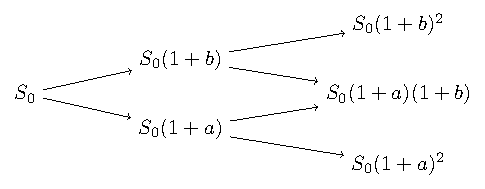
\includegraphics[width=.5\textwidth]{./stochv_abbildungen/stochv_1_2_crr}
		\captionof{figure}{Cox-Ross-Rubinstein-Modell}
		&
		$\hookrightarrow$ rekombinierender Baum, \newline
		Ereignisse $\omega$ entsprechen Pfaden im Baum
	\end{tabularx}	
\end{beispiel}

\begin{beispiel}[Black-Scholes-Modell, zeitstetig]
	Beim Black-Scholes-Modell handelt es sich um ein zeitstetiges Modell auf einem unendlichen Wahrscheinlichkeitsraum.
	\begin{equation*}
		\begin{aligned}
		S_t^0 &= e^{rt} && (\text{Verzinsung mit konstanter Rate } r) \\
		S_t^1 &= S_0^1 * \exp\brackets{(\mu-\frac{\sigma^2}{2}) + \sigma B_t} &&\mit \mu \in \R, \sigma > 0, S_0^1 > 0
		\end{aligned}
	\end{equation*}
	Der Term $\mu-\frac{\sigma^2}{2}$ beschreibt dabei eine Trendkomponenten, $B_t$ eine ''Brownsche Bewegung`` (zeitstetiger Prozess).
	\begin{center}
		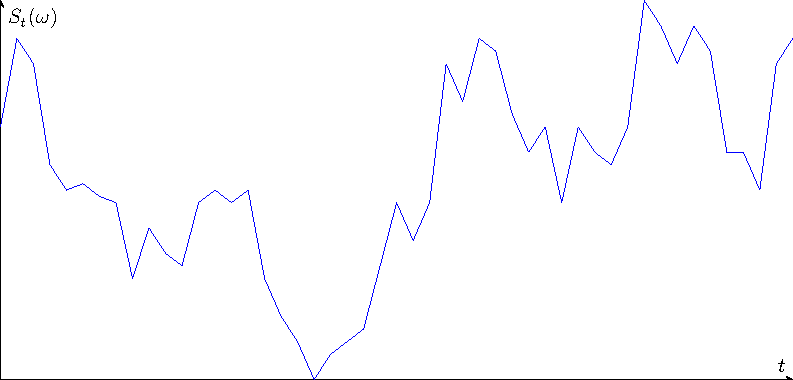
\includegraphics[width=.5\textwidth]{./stochv_abbildungen/stochv_1_2_bsm}
		\captionof{figure}{Black-Scholes-Modell}
	\end{center}
\end{beispiel}


\section{Anleihen und grundlegende Beispiele für Derivate}

Hier betrachten wir immer nur ein Basisgut $S_t = S_t^1$.

\begin{enumerate}[leftmargin=*, label=(\alph*)]
	\item \begriff{Anleihe} [bond] (genauer: Null-Kupon-Anleihe [zero-coupon bond])
	
	Der Emittent (Herausgeber) einer Anleihe mit Endfälligkeit [maturity] $T$ garantiert dem Käufer zum Zeitpunkt $T$ den Betrag $N$ (EUR/USD/...) zu zahlen.
	Typische Emittenten sind z.B. Staaten [government bond] oder Unternehmen (als Alternative zur Kreditaufnahme).
	Nach Emission werden Anleihen auf dem Sekundärmarkt weiterverkauft, d.h. liquide gehandelte Wertpapiere. 
	
	\begin{tabular}{ll}
		Preis bei Emission: & $B(0,T)$ \\
		Preis bei Weiterverkauf zum Zeitpunkt $t \le T$: & $B(t,T)$ \\
	\end{tabular}
	
	Es ist $B(T,T) = N$ und wir normieren stets $N=1 \follows B(T,T)=1$.
	
	Anleihen von West-/ Nord-/ Mitteleuropäischen Staaten und den USA sowie Kanada werden als risikolos betrachtet (sichere Zahlung). Sonst: Kreditrisiko
	
	Risikofreie Anleihen können als Numeraire $S_t^0 = B(t,T)$ genutzt werden.
	
	\begin{center}
		%TODO BILD (1)
		\includegraphics[width=.5\textwidth]{example-image}
		\captionof{figure}{Zahlungsstrom einer Anleihe}
	\end{center}
	
	\item \begriff{Terminvertrag} [forward contract]
	
	aus Käufersicht: Vereinbarung zu bestimmtem zukünftigen Zeitpunkt $T$ eine Einheit des Basisguts $S$ zum Preis $K$ zu kaufen (Kaufverpflichtung). Beliebt ist dieser bei Rohstoffen und Elektrizität.
	
	Auszahlungsprofil: $F_T = S_T - K$
	Preis zum Zeitpunkt $t$: $F_t$
	
	\begin{center}
		%TODO BILD (2)
		\includegraphics[width=.5\textwidth]{example-image}
		\captionof{figure}{Auszahlungsprofil eines Terminvertrags}
	\end{center}
	
	
	\item \begriff{(Europäische) Put- bzw. Call-Option}
	
	Recht zu einem zukünftigen Zeitpunkt $T$ eine Einheit des Basisguts $S$ zum Preis $K$ zu verkaufen (put) bzw. zu kaufen (call)
	$\to$ keine Kaufverpflichtung !
	% Vergleich zum Terminvertrag: keine Pflicht
	
	Auszahlungsprofil:
	\begin{itemize}
		\item Call: $C_T = \begin{cases} S_T - K & S_T \ge K \\ 0 & S_T < K \end{cases} = \brackets{S_T - K}_+$
		%TODO Bild (3)
		\item Put: $P_T = \begin{cases} 0 & S_T \ge K \\ K - S_T & S_T < K \end{cases} = \brackets{K - S_T}_+$ 
		%TODO Bild (4)
	\end{itemize}

	\item \begriff{Amerikanische Put- bzw. Call-Option}
	
	wie Put/Call, aber mit Ausübung zu beliebigem Zeitpunkt $\tau \in [0,T]$.
	
	\begin{tabular}{ll}
		Preis zum Zeitpunkt $t$: & $P_t^{AM}$, $C_t^{AM}$ \\
		Auszahlungsprofil zum Zeitpunkt $\tau$: & $\brackets{S_\tau - K}_+$, $\brackets{K - S_\tau}_+$
	\end{tabular}
	
	Der Zeitpunkt $\tau$ muss im Allgemeinen als Lösung eines stochastischen Optimierungsproblems bestimmt werden (optimales Stopp-Problem).
\end{enumerate}
\section{Elementare Replikations- und Ar"-bitrage"-argumente}

Was können wir (mit elementaren Mitteln) über die ''fairen`` Preise $B(t,T), F_t, C_t, P_t$ aussagen?

Wir verwenden:

\begin{itemize}[topsep=-\parskip]
	\item \begriff{Replikationsprinzip}: zwei identische, zukünftige Zahlungsströme haben auch heute denselben Wert (ein Zahlungsstrom ''repliziert`` den anderen)
	\item \begriff{No-Arbitrage-Prinzip}: ''Ohne Kapitaleinsatz kann kein sicherer Gewinn ohne Verlustrisiko erzielt werden.`` (Arbitrage = risikofreier Gewinn)
	\item \begriff{Superreplikationsprinzip} (schwächere Form des Replikationsprinzips): Ist ein Zahlungsstrom in jedem Fall größer als ein anderer, so hat er auch heute den größeren Wert.
\end{itemize}

\begin{center}
	\begin{tabular}{|c|c|c|}
		\hline
		stark & Replikationsprinzip & eingeschränkt anwendbar \\
		$\downarrow$ & Superreplikationsprinzip & $\uparrow$ \\
		schwach & No-Arbitrage-Prinzip & immer anwendbar \\
		\hline
	\end{tabular}
\end{center}

\begin{lemma} % 1.1
	Für den Preis $C_T$ des europäischen Calls gilt:
	\begin{equation*}
		\brackets{S_t - K B(t,T)}_+ \le C_t \le S_t
	\end{equation*}
\end{lemma}
\begin{proof}
	untere Schranke: Für Widerspruch nehme an, dass $S_t - K B(t,T) - C_t = \epsilon > 0$.
	
	\begin{center}
		\begin{tabular}{|l|c|cc|} % Wert in T über rechte beide Spalten
			\hline \multirow{2}{*}{Portfolio} & \multirow{2}{*}{Wert in $t$} & \multicolumn{2}{c|}{Wert in $T$} \\
			&& $S_T \le K$ & $S_T > K$ \\ \hline \hline
			Kaufe Call & $C_t$ & $0$ & $S_T - K$ \\
			Verkaufe Basisgut & $-S_T$ & $-S_T$ & $-S_T$ \\
			Kaufe Anleihe & $\epsilon + K B(t,T)$ & $\frac{\epsilon}{B(t,T)} + K$ &  $\frac{\epsilon}{B(t,T)} + K$ \\ \hline
			$\Sigma$ & $0$ & $K - S_T + \frac{\epsilon}{B(t,T)} > 0$ & $\frac{\epsilon}{B(t,T)} > 0$ \\
			& kein Anfangskapital & \multicolumn{2}{c|}{sicherer Gewinn}\\ \hline
		\end{tabular}
	\end{center}

	Dies steht jedoch im Widerspruch zum No-Arbitrage-Prinzip. Somit ist $S_t - K B(t,T) \le C_T$. Außerdem ist $C_t \ge 0$, d.h. $C_t \ge \brackets{S_t - K B(t,T)}_+$.
	
	obere Schranke: $\nearrow$ Übung
\end{proof}

\begin{lemma}[Put-Call-Parität] % 1.2
	Für Put $P_t$, Call $C_t$ mit selbem Ausübungspreis $K$ und Basisgut $S_t$ gilt
	\begin{equation*}
		C_t - P_t = S_t - B(t,T) * K
	\end{equation*}
	%TODO Bild (5)
\end{lemma}
\begin{proof}
	Mit Replikationsprinzip:
	
	\begin{center}
		\begin{tabular}{|l|c|cc|}
			\hline 
			\multirow{2}{*}{Portfolio 1} & \multirow{2}{*}{Wert in $t$} & \multicolumn{2}{c|}{Wert in $T$} \\
			&& $S_T \le K$ & $S_T > K$ \\ \hline \hline
			Kaufe Call & $C_t$ & $0$ & $S_T - K$ \\
			Kaufe Anleihe & $K * B(t,T)$ & $K$ & $K$ \\ \hline
			Wert Portfolio 1 & $C_t + K * B(t,T)$ & K & $S_T$ \\ 
			\hline
		\end{tabular}
	\end{center}

	\begin{center}
		\begin{tabular}{|l|c|cc|}
			\hline 
			\multirow{2}{*}{Portfolio 2} & \multirow{2}{*}{Wert in $t$} & \multicolumn{2}{c|}{Wert in $T$} \\
			&& $S_T \le K$ & $S_T > K$ \\ \hline \hline
			Kaufe Put & $P_t$ & $K - S_T$ & $0$ \\
			Kaufe Basisgut & $S_t$ & $S_T$ & $S_T$ \\ \hline
			Wert Portfolio 2 & $P_t + S_t$ & $K$ & $S_T$ \\ 
			\hline
		\end{tabular}
	\end{center}

	Replikationsprinzip: $C_t + K * B(t,T) = P_t + S_t \follows C_t + P_t = S_t - K*B(t,T)$
\end{proof}
\section{Bedingte Erwartungswerte und Martingale}

\subsection{Bedingte Dichte und bedingter Erwartungswert}

Motivation: Gegeben seien zwei Zufallsvariablen $(X,Y)$ mit Werten in $\R^m \times \Rn$ und gemeinsamer Dichte $f_{XY}(x,y)$.

Aus Dichte $f_{XY}$ können wir ableiten:
\begin{itemize}
	\item $f_Y(y) \defeq \int_{\R^m} f_{XY}(x,y) \dx$, die Randverteilung von $Y$
	\item $S_y \defeq \menge{y \in \Rn : f_Y(y) > 0}$, der Träger von $Y$
\end{itemize}

\begin{definition}
	Die bedingte Dichte von $X$ bzgl. $Y$ ist definiert als
	\begin{equation*}
	f_{X|Y}(x,y) = \begin{cases}
	\frac{f_{XY}(x,y)}{f_Y(y)} & y \in S_y \\ 0 & \notin S_y
	\end{cases}
	\end{equation*}
\end{definition}

Betrachte folgende Problemstellung: Was ist die beste Vorhersage von $X$ gegeben eine Beobachtung $Y = y$?

Kriterium: Minimiere quadratischen Abstand bzw. das zweite Moment bzw. die $L_2$-Norm.

Vorhersage: messbare Funktion $\abb{g}{\Rn}{\R^m}, y \mapsto g(y)$.

\begin{equation}
\min\menge{\EW[(X-g(y))^2] : g \text{ messbar } \Rn \to \R^m} \tag{min-1} \label{eq: min-1}
\end{equation}

\begin{proposition} %1.3
	Wenn $(X,Y)$ eine gemeinsame Dichte besitzen und $\EW[\abs{X}^2] < \infty$ gilt, dann wird \eqref{eq: min-1} minimiert durch die bedingte Erwartung
	\begin{equation*}
	g(y) = \EW[X | Y=y] \defeq \int_{\R^m} x f_{X | Y}(x,y) \dx
	\end{equation*}
	Wir bezeichnen $ \EW[X | Y=y]$ als Erwartungswert von $X$ bedingt auf $Y=y$.
\end{proposition}

Allgemeiner gilt:

\begin{theorem} %1.4
	Seien $(X,Y)$ Zufallsvariablen mit gemeinsamer Dichte auf $\R^m \times \Rn$ und $\abb{h}{\R^m \times \Rn}{\R}$ messbar mit $\EW[h(X,Y)^2]$. Dann wird das Minimierungsproblem
	\begin{equation*}
	\min\menge{\EW[(h(X,Y)-g(Y))^2] : g \text{ messbar } \Rn \to \R}
	\end{equation*}
	gelöst durch
	\begin{equation*}
	g(y) = \EW[h(X,Y) | Y = y] = \int_{\R^m} h(x,y) * f_{X|Y}(x,y) \dx
	\end{equation*}
\end{theorem}

\begin{proof}[nur Proposition für $m=1$, Theorem analog]
	Setze $g(y) = \int_{\R} x f_{X|Y}(x,y) \dx$. Sei $\abb{p}{\Rn}{\R}$ eine beliebige messbare Funktion mit $\EW[p(Y)^2]< \infty$. Setze weiter $g_\epsilon(y) = g(y) + \epsilon p(y)$. Minimiere $F(\epsilon) \defeq \EW[(X-g_\epsilon(y))^2] = \EW[(X - g(y) - \epsilon p(y))^2] = \EW[(X-g(Y))^2] - 2\epsilon \EW[(X-g(Y)) p(Y)] + \epsilon^2 \EW[p(Y)^2]$.
	\begin{equation*}
	\begin{aligned}
	\frac{\partial F}{\partial \epsilon}(\epsilon) &= 2\epsilon \EW[p(Y)^2] - 2\EW[(X-g(Y)) p(Y)]  \follows \epsilon_\ast \defeq\frac{\EW[(X-g(Y))p(Y)]}{\EW[p(Y)^2]} = \frac{A}{B} \\
	A &= \EW[Xp(Y)] - \EW[g(Y) p(Y)]  \\
	&= \int_{\R \times \Rn} x p(y) f_{XY}(x,y) \dx \dy - \int_{S_y} g(y) p(y) f_Y(y) \dy \\
	&= \int_{\R \times \Rn} x p(y) f_{XY}(x,y) \dx \dy - \int_{\R \times S_y} x p(y) \underbrace{f_{X|Y}(x,y) f_Y(y)}_{=f_{XY}(x,y)} \dy = 0
	\end{aligned}
	\end{equation*}
	Damit ist $\epsilon^\ast = 0$ unabhängig von $p$ und $g(y)$ minimiert \eqref{eq: min-1}.
\end{proof}

\begin{*beispiel}
	Seien $(X,Y)$ normalverteilt auf $\R \times \R$ mit
	\begin{equation*}
	\mu = \begin{pmatrix} \mu_X \\ \mu_Y \end{pmatrix} \qquad \Sigma 
	= \begin{pmatrix} Var[X] & \Cov{X}{Y} \\ \Cov{X}{Y} & \Var[Y] \end{pmatrix}
	= \begin{pmatrix}
	\sigma_x^2 & \rho \sigma_x \sigma_y \\ \rho \sigma_x \sigma_y & \sigma_y^2
	\end{pmatrix}
	\qquad \rho \in [-1,1]
	\end{equation*}
	Dann ist die bedingte Dichte $f_{X|Y}(x,y)$ wieder die Dichte einer Normalverteilung mit
	\begin{equation*}
	\begin{aligned}
	\EW[X|Y=y] &= \mu_X + \rho \frac{\sigma_X}{\sigma_Y} \brackets{y - \mu_Y} \\
	\Var[X|Y=y] &= \sigma_X^2 (1-\rho^2)
	\end{aligned}
	\end{equation*}
	$\to$ siehe Übung.
	
	Die Abbildung $y \mapsto \mu_X + \rho \frac{\sigma_X}{\sigma_Y}(Y-\mu_Y)$ heißt Regressionsgerade für $X$ gegeben $Y = y$.
	
	% TODO Abbildung Regressionsgerade
	
	Die Steigung wird im Wesentlichen durch $\rho$ bestimmt.
	
	Für diskrete Zufallsvariablen, d.h. wenn $X$,$Y$ nur endliche viele Werte $\menge{x_1, \dots , x_m}$ bzw. $\menge{y_1, \dots, y_n}$ annehmen, dann erhalten wir mit ähnlichen Überlegungen als Lösung von \eqref{eq: min-1} 
	\begin{equation*}
	\EW[X | Y=y_j] = \sum_{i=1}^m x_i \P(X=x_i | Y=y_j)
	\end{equation*}
	wobei direkt die bedingten Wahrscheinlichkeiten
	\begin{equation*}
	\P(X=x_i | Y=y_j) = \begin{cases}
	\frac{\P(X=x_i \land Y = y_j)}{\P(Y=y_j)} & \text{wenn } \P(Y = y_j) > 0 \\
	0 & \text{wenn } \P(Y=y_j) = 0
	\end{cases}
	\end{equation*}
	folgen.
\end{*beispiel}

\subsection{Bedingte Erwartung: Maßtheoretischer Zugang}

Wir betrachten den Wahrscheinlichkeitsraum $(\Omega, \F, \P)$. Für eine Zufallsvariable $\abb{X}{\Omega}{\R}$ und $p \in [1,\infty)$ definieren wir, doe $L_p$-Norm
\begin{equation*}
\norm{X}_p \defeq \EW[\abs{X}^p]^{\frac{1}{p}} = \brackets{\int_\Omega \abs{X(\omega)}^p \diffskip{\P(\omega)}}^\frac{1}{p}
\end{equation*}
und den $L_p$-Raum
\begin{equation*}
L_p(\Omega, \F, \P) \defeq \menge{\abb{X}{\Omega}{\R} \enskip \F\text{-messbar}, \norm{X}_p < \infty}
\end{equation*}
Dabei identifizieren wir Zufallsvariablen, die sich nur auf $\P$-Nullmengen unterscheiden miteinander, d.h. $\P(X \neq X') = 0 \follows X = X'$ in $L_p$. Aus der Maßtheorie bekannt: Die Räume $L_p(\Omega,\F,\P)$ mit Norm $\norm{\dots}_p$ mit $p \in [1,\infty)$ sind
\begin{itemize}
	\item Banachräume, d.h. vollständige, normierte Vektorräume.
	\item für $p=2$ auch Hilbertraum mit inneren Produkt 
	\begin{equation*}
	\scal{X}{Y} = \EW[XY] = \int_\Omega X(\omega) Y(\omega) \diffskip{\P(\omega)}
	\end{equation*}
\end{itemize}

Für $\G \subseteq \F$ Unter-$\sigma$-Algebra ist $L_p(\Omega,\G,\P) \subseteq L_p(\Omega, \F, \P)$ ein abgeschlossener Unterraum.

Wir verallgemeinern das ''Vorhersageproblem`` ais dem letzten Abschnitt: Gegeben sei ein Zufallsvariale $X$ aus $L_2(\Omega,\F,\P)$ und $\G \subseteq \F$ eine Unter-$\sigma$-Algebra. Was ist die beste $\G$-messbare Vorhersage für $X$?

\begin{equation}
\min\menge{\EW[(X-G)^2] : G \in L_2(\Omega,\G,\P)} \tag{min-2} \label{eq: min-2}
\end{equation}

Aus Hilbertraumtheorie folgt, dass \eqref{eq: min-2} besitzt eine eindeutige Lösung $G_\ast \in L_(\Omega, \G, \P)$. $G_\ast$ ist die Orthogonalprojektion (bzgl. $\scal{\cdot}{\cdot}$) von $X \in L_2(\Omega,\F,\P)$ auf den abgeschlossenen Unterraum $L_2(\Omega,\G,\P)$.

% TODO Abbildung Hilbertraum

Wir bezeichnen $G_\ast$ mit $\EW[X|\G]$ als bedingten Erwartunswert von $X$ bezüglich $\G$.

\begin{theorem} %1.5 
%	\label{theorem: 1.5}
	SSeien $X,Y \in L_2(\Omega,\F,\P)$ und $\G \subseteq \F$ eine Unter-$\sigma$-Algebra. Dann gilt
	\begin{itemize}
		\item Linearität: $\EW[aX + bY | \G] = a \EW[X|\G] + b\EW[Y|\G]$
		\item Turmregel: Für jede weitere $\sigma$-Algebra $\mathcal{H} \subseteq \G$ gilt ${\EW[{\EW[{X|\G}]}|\mathcal{H}]} = {\EW[X|\mathcal{H}]}$
		\item Pull-out-Property: $\EW[XZ|\G] = Z * \EW[X | \G]$ für alle beschränkten und $\G$-messbaren Zufallsvariablen $Z$.
		Für $Z$ $\G$-messbar mit $\EW[\abs{XZ}] < \infty$ gilt $\EW[XZ | \G] = Z * \EW[X | \G]$. Insbesondere gilt für $\G$-messbare $X$ schon $\EW[X|\G]=X$.
		\item Monotonie: $X \le Y \follows \EW[X|\G] \le \EW[Y|\G]$
		\item Dreiecksungleichung: $\abs{\EW[X|\G]} \le \EW[\abs{X}|\G]$
		\item Unabhängigkeit: $X$ unabhängig von $\G$ $\follows$ $\EW[X|\G] = \EW[X]$
		\item triviale $\sigma$-Algebra: $\G=\menge{\emptyset, \Omega} \follows \EW[X|\G] = \EW[X]$
	\end{itemize}
\end{theorem}
\begin{proof}
	siehe VL ''Wahrscheinlichkeitstheorie mit Martingalen``
\end{proof}

Die für $X \in L_2(\Omega,\F,\P)$ definierte bedingte Erwartung $\EW[X|\G]$ lässt sich durch Approximation auf alle $X \in L_1(\Omega,\F,\P)$ erweitern. Alle Eigenschaften aus Theorem 1.5 bleiben erhalten. %TODO Ref

Sei $Y$ eine Zufallsvariable und $\G= \sigma(Y)$ die von $Y$ erzeugte $\sigma$-Algebra. Wir schreiben $\EW[X|Y] = \EW[X|\sigma(Y)]$; dies ist eine $\G$-messbare Zufallsvariable.

Aus der Maßtheorie sag uns das Doob-Dynkin-Lemma, dass eine messbare Funktion $\abb{g}{\Rn}{\R}$ existiert, sodass $\EW[X|Y] = g(Y)$. Dabei ist $g$ genau die Funktion aus \eqref{eq: min-1}.

Zusammenfassung

Sei $X,Y$ aus $L_1(\Omega,\F,\P)$ und $\G \subseteq \F$ eine Unter-$\sigma$-Algebra. 
\begin{enumerate}[label=(\alph*),nolistsep,topsep=-\parskip]
	\item $\EW[X|Y=y]$ ist eine messbare Funktion $\abb{g}{\Rn}{\R^m}$ und falls eine bedingte Dichte existiert, dann gilt $\EW[X|Y=y] = \int_{\R^m} x f_{X|Y}(x,y) \dx$.
	\item $\EW[X|Y]$ ist eine $\sigma(Y)$-messbare Zufallsvariable und kann als $g(Y)$ dargestellt werden. Falls eine bedingte Dichte existiert, dann gilt $\EW[X|Y](\omega) = \int_\Rn x f_{X|Y}(x,Y(\omega)) \dx$.
	\item $\EW[X|\G]$ ist eine $\G$-messbare Zufallsvariable. Falls $\G=\sigma(Y)$ tritt Fall (b) ein.
\end{enumerate}
In allen Fällen kann $\EW[X|\cdot]$ interpretiert werden als \textit{beste Vorhersage} für $X$ gegeben
\begin{enumerate}[label=(\alph*),nolistsep,topsep=-\parskip]
	\item eine punktweise Betrachtung $Y=y$
	\item die Beobachtung $Y$
	\item die Information $\G$
\end{enumerate}

\subsection{Martingale}

Prototyp eines ''neutralen`` stochastischen Prozesses, der weder Aufwärts- noch Abwärtstrend besitzt. Wir betrachten hier den Prozess nur in diskreter Zeit $I = \N_0$.

\begin{definition}
	Sei $\folge{X}{n \in \N_0}$ ein stochastischer Prozess. Wenn gilt
	\begin{equation}
	\begin{alignedat}{2}
		\EW[\abs{X_n}] &< \infty \qquad &\forall n \in \N \\
		\EW[X_{n+1}|X_1,\dots,X_n] &= X_n \qquad &\forall n \in \N \\
	\end{alignedat}
	\end{equation}
	dann heißt $\folge{X_n}{n \in \N}$ \begriff{Martingal}.
\end{definition}

Wenn wir $\F_n^X = \sigma(X_1,\dots,X_n)$ definieren, können wir (b) schreiben als 
\begin{equation*}
	\EW[X_{n+1}|\F_n^X] = X_n \qquad \forall n \in \N
\end{equation*}

\textbf{Konvention}: Alle stochastischen Prozesse $\folge{X_n}{n \in \N_0}$ haben deterministischen Startwert $X_0$.

Interpretation: Beste Vorhersage für zukünftigen Wert $X_{n+1}$ basierend auf Vergangenheit $\sigma(X_1,\dots,X_n)$ ist der momentane Wert $X_n$.
Aus der Turmregel folgt:
\begin{equation*}
	\EW[X_{n+k}|\F_n^X] = X_n \qquad \forall n,k \in \N_0 %b''
\end{equation*}
denn
\begin{equation*}
	\EW[X_{n+k}|\F_n^X] = \EW[\underbrace{\EW[X_{n+k}|\F_{n+k-1}^X]}_{=X_{n+k-1}}|\F_n^X] = \EW[X_{n+k-1}|\F_n^X] \overset{k \text{ mal}}{=} X_n
\end{equation*}

Man kann von $\folge{\F_n^X}{n \in \N}$ auf beliebige Filtrationen $\folge{\F_n}{n \in \N_0}$ erweitert werden.

\begin{*definition}
	Sei $\folge{X_n}{n \in \N_0}$ ein stochastischer Prozess, adaptiert an eine Filtration $\folge{\F_n}{n \in \N_0}$. Wenn gilt
	\begin{alignat*}{2}
		\EW[\abs{X_n}] &< \infty &\forall n \in \N_0 \\ % (a)
		\EW[X_{n+1}|\F_n] &= X_n &\forall n \in \N_0    % (b)
	\end{alignat*}
	dann heißt $\folge{X_N}{n \in \N}$ Martingal bezüglich der Filtration $\folge{\F_n}{n \in \N}$.
\end{*definition}

Interpretation: Beste Vorhersage für zukünftigen Wert $X_{n+1}$, basierend auf verfügbarer Information $\F_n$ ist der momentane Wert $X_n$.

\begin{*definition}
	Falls in Punkt (b) statt ''$=$`` die Ungleichung ''$\le$`` oder ''$\ge$`` gilt, so heißt $\folge{X_n}{n \in \N}$ \begriff{Super- bzw. Submartingal}.
\end{*definition}

\begin{itemize}
	\item Wenn $X=\folge{X_n}{n \in \N}$ ein Martingal ist, dann gilt $\EW[X_n] = X_0$, d.h. $n \mapsto \EW[X_n]$ ist konstant. Begründung:
	\begin{equation*}
	\EW[X_{n+1}|\F_n] = X_n \follows \underbrace{\EW[{\EW[X_{n+1}|\F_n]}]}_{= \EW[X_{n+1}]} = \EW[X_n] \overset{n \text{ mal}}{\follows} \EW[X_n] = X_0
	\end{equation*}
	\item $X$ Submartingal $\follows n \mapsto \EW[X_n]$ ist monoton steigend
	\item $X$ Supermartingal $\follows n \mapsto \EW[X_n]$ ist monoton fallend
\end{itemize}

''Das Leben ist ein Supermartingal -- die Erwartungen fallen mit der Zeit`` \smiley

\begin{beispiel}
	\begin{itemize}
		\item Seien $\folge{Y_n}{n \in \N}$ unabhängige Zufallsvariablen in $L_1(\Omega,\F,\P)$ mit $\EW[Y_n] = 0$. Betrachten wir die Partialsummen $X_n \defeq \sum_{k=1}^n Y_k$ und $X_0 = 0$. Dann ist $\folge{X_n}{n \in \N_0}$ ein Martingal, denn
		\begin{equation*}
			\begin{aligned}
			\EW[\abs{X_n}] &\le \sum_{k=1}^n \EW[\abs{Y_k}] < \infty \qquad \forall n \in \N \\
			\EW[X_{n+1} \mid \F_n^X] &= \EW[Y_{n+1} + X_n \mid \F_n^X] \\
			&= \EW[y_{n+1} \mid \F_n^X] + \EW[X_n \mid \F_n^X] = \underbrace{\EW[Y_{n+1}]}_{=0} + X_n \\
			&= X_n
			\end{aligned}
		\end{equation*}
	\end{itemize}
\end{beispiel}

\begin{*definition}
	Sei $\folge{\F_n}{n \in \N_0}$ eine Filtration. Ein stochastischer Prozess $\folge{H_n}{n \in \N}$ heißt \begriff{vorhersehbar} [predictable] bezüglich $\folge{\F_n}{n \in \N_0}$ wenn gilt
	\begin{equation*}
		H_n \text{ ist } \F_{n-1} \text{-messbar} \qquad \forall n \in \N
	\end{equation*}
\end{*definition}

\begin{*bemerkung}
	Vorhersehbarkeit ist eine stärkere Eigenschaft als Adaptiertheit.
\end{*bemerkung}

\begin{*definition}
	Sei $X$ ein adaptierter und $H$ ein vorhersehbarer stochastischer Prozess bezüglich $\folge{\F_n}{n \in \N}$. Dann heißt 
	\begin{equation}
		(H \bullet X)_n \defeq \sum_{k=1}^n H_k (X_k - X_{k-1}) \tag{$\star$} \label{eq: diskretesIntegral}
	\end{equation}
	\begriff{diskretes stochastisches Integral} von $H$ bezüglich $X$.
\end{*definition}

\begin{*bemerkung}
	Summen \eqref{eq: diskretesIntegral} heißen in der Analysis Riemann-Stieltjes-Summen und werden für die Konstruktion des Riemann-Stieltjes-Integrals $\int h \diffskip{\rho}$ verwendet.
\end{*bemerkung}

\begin{*definition}
	Ein stochastischer Prozess $\folge{H_n}{n \in \N}$ heißt lokal beschränkt, wenn eine deterministische Folge $c_n \in \R_{\ge 0}$ existiert, sodass
	\begin{equation*}
		\abs{H_n} \le c_n \enskip \text{ fast sicher } \qquad \forall n \in \N
	\end{equation*}
\end{*definition}

\begin{satz} %1.6
	Sei $X$ adaptierter stochastischer Prozess (bezüglich Filtration $\folge{\F_n}{n \in \N}$). Dann sind äquivalent:
	\begin{enumerate}
		\item $X$ ist Martingal bezüglich $\folge{\F_n}{n \in \N}$.
		\item $(H \bullet X)$ ist Martingal für alle lokal beschränkten, vorhersbaren Prozesse $H$
	\end{enumerate}
\end{satz}

Das heißt, dass das stochastische Integral die Martingaleigenschaft erhält.

\begin{proof_equiv}
	\hinrichtung $(H \bullet X)_n = \sum_{k=1}^n H_k (X_k - X_{k-1})$.
	\begin{itemize}
		\item Adaptiertheit: klar
		\item Integrierbarkeit: $H$ lokal beschränkt, d.h. $\abs{H_k} \le c_k < \infty$ für alle $k$.
		\begin{equation*}
			\EW[\abs{H_k (X_k - X_{k-1})}] \le c_k * \brackets{\EW[\abs{x_k}] + \EW[\abs{X_{k+1}}]} < \infty
		\end{equation*}
		Mit der Dreiecksungleichung folgt daraus $\EW[\abs{(H \bullet X)_n}] < \infty$.
		\item Martingaleigenschaft: 
		\begin{equation*}
			\EW[(H \bullet X)_n \mid \F_{n-1}] = (H \bullet X)_{n-1} + \EW[H_n (X_n - X{n-1}) \mid \F_{n-1}]
			=  (H \bullet X)_{n-1} + H_n * \underbrace{\brackets{\EW[X_n \mid \F_{n-1}] - X{n-1}}}_{=0} 
			=(H \bullet X)_{n-1} \quad \forall n \in \N
		\end{equation*}
		Damit ist also auch $(H \bullet X)$ ein Martingal.		
	\end{itemize}
	\rueckrichtung Fixiere $N \in \N$. Setze $H_n \defeq \one_{n = N}$, dieser ist lokal beschränkt und deterministisch (also auch vorhersehbar). Man stellt fest, dass $(H \bullet X)_n = 0$ für alle $n \le N-1$. Für alle $n \ge N$ gilt dagegen $(H \bullet X)_n = X_N - X_{N-1}$. Wir überprüfen nur die Martingaleigenschaft (Integrierbarkeit folgt aus Dreiecksungleichung). Wir wissen, dass $(H \bullet X)$ ein Martingal ist. 
	\begin{align*}
		0 = (H \bullet X)_{N-1} = \EW[(H \bullet X)_N \mid \F_{N-1}] = 
		\EW[x_N - X_{N-1} \mid \F_{N-1}] = \EW[X_N \mid \F_{N-1}] - X_{N-1}
		\follows X_{N-1} = \EW[X_N \mid \F_{N-1}] \mit N \in \N \text{beliebig}
	\end{align*}
	Somit ist $X$ ein Martingal.
\end{proof_equiv}

\begin{korollar} %1.7
	Sei $X = \folge{X_n}{n=1 , \dots, N}$ ein adaptierter stochastischer Prozess bezüglich einer Filtration $\folge{\F_n}{n=1 , \dots, N}$. Wenn $\EW[(H \bullet X)_N] = 0$ für alle lokal beschränkten vorhersehbaren Prozesse $H$, dann ist $X$ ein Martingal bezüglich $\folge{\F_n}{}$.
\end{korollar}
\begin{proof}
	Fixiere $K \in  [N] \defeq \menge{1, 2, \dots , N}$ und eine Menge $A \in \F_{K-1}$. Definiere $H_n(\omega) = \one_A (\omega) * \one_{\menge{n=K}}$, dieser ist lokale beschränkt und vorhersehbar.
	Es ist $(H \bullet X)_n = 0$ für alle $n \le K-1$. Für alle $n \ge K$ gilt $(H \bullet X)_n = \one_A * (X_K - X_{K-1})$. 
	\begin{align*}
%	0 = \EW[(H \bullet X)_N] = \EW[\one_A (X_K - X_{K-1})] 
%	\overset{Turm}{=} \EW[\EW[\one_A (X_K - X_{K-1}) \mid \F_{K-1}]] 
%	= \EW[\one_A * \brackets{\underbrace{\EW[X_K \mid \F_{K-1] - X_{K-1}}]}_{\defqe Y_{K-1}}} \quad \forall A \in \F_{K-1}
%		\follows \int_A  Y_{K-1}(\omega) \diff{\P(\omega)} = \int_A X_{K-1}(\omega) \diff{\P(\omega)} \quad \forall A \in \F_{K-1}
%		\follows Y_{K-1} = X_{K-1} fast sicher
%		\follows \EW[X_K \mid \F_{K-1] - X_{K-1}}] = X_{K-1}
	\end{align*}
	für beliebige $K$. Somit ist $X$ ein Martingal.
\end{proof}

\begin{bemerkung}
	Wir schreiben $[N] \defeq \menge{1, 2, \dots, N}$ und $[N]_0 \defeq \menge{0, 1, 2 , \dots , N}$.
\end{bemerkung}


\chapter{Cox-Ross-Rubinstein-Modell}
\label{chapter_2_crr}
Das Cox-Ross-Rubinstein-Modell (kurz: CRR-Modell) wird auch Binomialmodell genannt und wurde 1979 von Cox, Ross und Rubinstein entwickelt.

Es handelt sich dabei um ein Modell für die Preisentwicklung eines Wertpapiers plus ein Verrechnungskonto mit konstanter Verzinsung (Numeraire) in diskreter Zeit.

\textbf{Parameter:}

\begin{center}
	\begin{tabular}{|c|l|}
		\hline
		$r$ & Zinsrate \\ \hline
		$b$ & Rendite des Wertpapiers bei Aufwärtsbewegung (''up``) \\ \hline
		$a$ & Rendite des Wertpapiers bei Abwärtsbewegung(''down``) \\ \hline
		$p \in (0,1)$ & Wahrscheinlichkeit für ''up`` \\ \hline
		$S_0 > 0$ & Preis Wertpapier zum Zeitpunkt Null \\ \hline
		$N \in \N$ & Anzahl der Zeitschritte \\ \hline
	\end{tabular}
\end{center}

\textbf{Annahmen:} $r > -1$, $b > a > -1$

Wir modellieren Wertpapiere $\folge{S_k}{k \in [N]}$ und Verrechnungskonto $\folge{S_k^0}{k \in \N}$ als stochastische Prozesse auf einem Wahrscheinlichkeitsraum $(\Omega, \F, \P)$.

\begin{itemize}
	\item $S_0^0 = 1$ und $S_n^0 = (1+r)^n$
	\item Wir definieren die \begriff{Rendite} $R_n(\omega)$ in der $n$-ten Marktperiode durch
	\begin{equation*}
		R_n = \begin{cases} b & \mit p \\ a & \mit 1-p \end{cases}
	\end{equation*}
	Die Renditen $(R_1, \dots, R_N)$ sind unabhängig.
	\begin{equation*}
		S_n = S_0 * \prod_{k=1}^n (1+R_k)
	\end{equation*}
	
	Der Verlauf von $S$ lässt sich grafisch als Binomialbaum darstellen:
	
	\begin{center}
		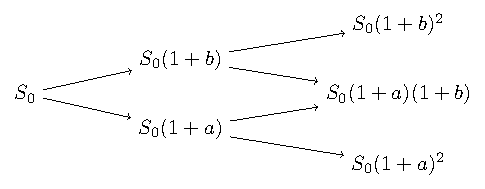
\includegraphics[width=.5\textwidth]{stochv_abbildungen/stochv_1_2_crr.pdf}
	\end{center}
	
	Man nennt dies auch ein ''rekombinierendes Baummmodell``. Es hat den Vorteil, dass die Anzahl der Knoten nur linear mit $n$ wächst.
	
	\item Abgezinster Preisprozess $\schlange{S}_n \defeq \frac{S_n}{S_n^0} = S_0 * \prod_{k=1}^n \frac{1+R_k}{1+r}$.
	
	\item Filtration: natürliche Filtration $\F_n = \sigma \brackets{S_1, \dots, S_n}$.
\end{itemize}

\begin{proposition} %2.1
	Im CRR-Modell gilt:
	\begin{enumerate}[label=(\alph*)]
		\item Die Anzahl der Aufwärtsbewegungen $U_n \defeq \# \menge{k \in [n] \colon R_k = b}$ ist binomialverteilt, d.h. $U_n \sim \Bin(n,p)$.
		\item Es gilt 
		\begin{equation*}
			\log\brackets{\frac{\schlange{S}_n}{S_0}} = U_n \log\brackets{\frac{1+b}{1+a}} + n \log\brackets{\frac{1+a}{1+r}}
		\end{equation*}
		d.h. $\log\brackets{\frac{\schlange{S}_n}{S_0}}$ ist nach Skalen-Lagen-Transformation binomialverteilt.
		\item Die Verteilung von $S_n$ ist gegeben durch
		\begin{equation*}
			\P\brackets{S_n = S_0 (1+b)^k (1+a)^{n-k}} = \binom{n}{k} p^k (1-p)^{n-k}
		\end{equation*} 
	\end{enumerate}
\end{proposition}

\begin{proof}
	\begin{enumerate}[label=(zu \alph*), leftmargin=\zulength]
		\item klar
		\item $\frac{\schlange{S}_n}{S_0} = \brackets{\frac{1+b}{1+a}}^{U_n} * \brackets{\frac{1+a}{1+r}}^n \follows \log\brackets{\frac{\schlange{S}_n}{S_0}} = U_n \log\brackets{\frac{1+b}{1+a}} + n \log\brackets{\frac{1+a}{1+r}}$
		\item Es ist $S_n = S_0 (1+b)^{U_1}(1+a)^{n-U_n} $. Also
		\begin{equation*}
			\P\brackets{S_n = S_0 (1+b)^k (1+a)^{n-k}} = \P(U_n = k) \overset{(a)}{=} \binom{n}{k} p^k (1-p)^{n-k}
		\end{equation*}
	\end{enumerate}
\end{proof}

\begin{*bemerkung_inline}
	Teil (b) suggeriert Konvergenz von $\log\brackets{\frac{\schlange{S}_n}{S_0}}$ gegen Normalverteilung für $n \to \infty$ (nach Skalierung) 
	$\leadsto$ Black-Scholes-Modell ($\nearrow$ Kapitel 3).
\end{*bemerkung_inline}
\section{Anlagestrategien im CRR-Modell}

Eine Anlagestrategie soll durch ein Anfangskapital $w$ und einen stochastischen Prozess $\folge{\eta_n, \xi_n}{n \in [N]}$ dargestellt werden. 
\begin{itemize}
	\item Dabei steht $\xi_n$ für die ''Anzahl`` der Wertpapiere, die im Zeitintervall $(n-1,n]$ gehalten werden. Negative Werte von $\xi_n$ sind sogenannte Leerverkäufe. Wir erlauben beliebige Anteile $\xi_n \in \R$.
	\item Weiter beschreibt $\eta_n$ den Stand des Verrechnungskontos in Geldeinheiten zum Zeitpunkt Null. Negative Werte von $\eta_n$ entsprechend einer Kreditaufnahme.
	Außerdem sei das Anfangskapital $w \in \R$.
\end{itemize}

\textbf{\underline{Gesamtwert des Portfolios}}

\begin{equation*}
\begin{aligned}
\Pi_n &= \eta_n * S_n^0 + \xi_n * S_n \\
\Pi_0 &= w
\end{aligned} \tag{Port} \label{eq: port}
\end{equation*}
Man nennt \eqref{eq: port} die \begriff{Portfoliogleichung}.

Annahmen an die Strategie:
%\begin{itemize}
%	\item Die Strategie darf nur von Beobachtungen der Vergangenheit abhängen, d.h. $(\eta_n, \xi_n)$ ist ein \textit{vorhersehbarer} Prozess.
%	\item Portfolio wird nur zwischen $S$ und $S_0$ umgeschichtet, d.h. es wird kein Kapital zugeschossen oder abgezogen.
%	
%	$\Pi_n = \eta_n S_n^0 + \xi_n S_n$ Wert zum Zeitpuntk $n$ vor dem Umschichten
%	$\Pi_n = \eta_{n+1} S_n^0 + \xi_{n+1}S_n$ Wert zum Zeitpunkt $n$ nach dem Umschichten
%	$\Pi_{n+1} = \eta_{n+1} S_{n+1}^0 + \xi_{n+1} S_{n+1}$ Wert zum Zeitpunkt $n+1$ vor dem Umschichten.
%	Subtrahiere Gleichung 2 und 3
%	$\follows \Pi_{n+1} - \Pi_n = \eta_{n+1} \brackets{S_{n+1}^0 - S_n^0} + \xi_{n+1} \brackets{S_{n+1} - S_n}$
%	kurz: $\Delta \Pi_n = \eta_n \Delta S_n^0 + \xi_m \Delta S_n$ (Selbstfinanzierungseigenschaft, SF)
%	beachte: $\Delta \Pi_n \defeq \Pi_n - \Pi_{n-1}$
%	
%	Diskontieren: $\schlange{\Pi_n} = \frac{\Pi_n}{S_n^0}$ ... diskontierter Portfoliogleichung
%	Wier erhalten aus (Port)
%	$\schlange{\Pi_n} = \eta_n + \xi_n \schlange{S}_n$
%	$\schlange{\Pi_0} = w$ (Port schlange)
%	
%	Aus (SF)
%	$\Delta \schlange{\Pi_n} = \xi_n \Delta \schlange{S}_n$ (SF Schlange)	
%	
%	d.h. $\schlange{\Pi}_n  = w + \sum_{k=1}^n \brackets{\schlange\Pi_k - \schlange\Pi_{k-1} \overset{(SF)}{=} w + \sum_{k=1}^n \xi_k \brackets{\schlange S_k - \schlange S_{k-1}} = w + \brackets{\xi \bullet \schlange{S}}_n$
%		
%	$\schlange\Pi_n = w + \brackets{\xi \bullet \schlange{S}}_n$ (INt Schlange)
%\end{itemize}
\section{Replikation / Hedging von Derivaten im CRR-Modell}

Derivat $C$ mit Auszahlung $h(S_1, S_2, \dots, S_N)$ zum Zeitpunkt $N$, d.h. $C = h(S_1, S_2, \dots, S_N)$ mit $h$ messbar

Gesucht ist nun eine replizierende Strategie $\folge{\xi_n}{n \in \N}$ und eine Anfangskapital $w$, d.h.
\begin{itemize}[label = --, nolistsep, topsep=-\parskip]
	\item $\folge{\xi_n}{n \in \N}$ soll vorhersehbar sein mit diskontiertem Werteprozess $\schlange{\Pi}_n = w + (\xi \bullet \schlange{S})_n$ und 
	\item die Replikationsbedingung soll gelten
	\begin{equation*}
	C = h(S_1, \dots, S_N) = \Pi_N  \qquad \text{fast sicher} \tag{Rep} \label{eq: 2_2_rep}
	\end{equation*}
\end{itemize} 

\begin{*definition}
	\begin{itemize}[nolistsep, topsep=-\parskip]
		\item Ein Derviat $C$ heißt \begriff{erreichbar}, wenn eine Replikationsstrategie existiert.
		\item Ein Finanzmarktmodell heißt \begriff{vollständig}, wenn jedes Derivat erreichbar ist.
	\end{itemize}
\end{*definition}

\begin{satz} %2.3
	\label{satz: 2.2.3}
	Sei $C = h(S_1, \dots, S_N)$ ein Derivat im CRR-Modell. Dann ist $C$ erreichbar, d.h. es existieren $w \in \R$ und $\folge{\xi_n}{n \in \N}$ mit \eqref{eq: 2_2_rep}. Es gilt:
	\begin{itemize}
		\item Es existieren messbare Funktionen $\abb{f_n}{\Rn}{\R}$ für $n =1, \dots, N$, sodass
		\begin{equation*}
			\Pi_n = f_n(S_1, \dots, S_n)
		\end{equation*}
		und die Werte entlang der Pfade des Binomialbaums sind rekursiv bestimmt:
		\begin{align*}
				f_N(S_1, \dots, S_N) &= h(S_1, \dots, S_N) = C \\
				f_n(S_1, \dots, S_n) &= \frac{1}{1+r} \brackets{\frac{r-a}{b-r} f_{n+1}^b + \frac{b-r}{b-a} f_{n+1}^a} \text{ wobei } \tag{Rek} \label{eq: 2_2_rek}
			\intertext{wobei}
				f_{n+1}^b &= f_{n+1}(S_1, \dots, S_n, S_n (1+b)) \\
				f_{n+1}^a &= f_{n+1}(S_1, \dots, S_n, S_n (1+a))  \qquad n \in [N]_0
		\end{align*}		
		\item Die replizierende Strategie ist gegeben durch 
		\begin{equation*}
			\xi_n = \frac{f_n^b - f_n^a}{S_{n-1} (b-a)} \tag{$\Delta$-Hedge} \label{eq: 2_2_dhedge}
		\end{equation*}
	\end{itemize}
\end{satz}

\begin{korollar} %2.4
	Das CRR-Modell ist vollständig.
\end{korollar}

\begin{korollar} %2.5
	Ist $C$ ein europäisches Derivat, d.h. $C = h(S_N)$ mit $\abb{h}{\R}{\R}$ messbar, dann gelten folgende Vereinfachungen: Es reicht $\abb{f_n}{\R}{\R}$ zu wählen und es gilt $\Pi_n = f_n(S_n)$ sowie
	\begin{equation*}
		f_{n+1}^b = f_{n+1}(S_n (1+b)) \quad \und \quad f_{n+1}^a = f_{n+1}(S_n(1+a))
	\end{equation*}
\end{korollar}

\begin{*bemerkung}
	\begin{itemize}[leftmargin=*, label=$\bullet$, nolistsep]
		\item Die Rekursion \eqref{eq: 2_2_rek} entspricht einem Rückwärtsdurchlauf des Baumdiagramms.$f_n$ wird als diskontierter, gewichteter Mittelwert von $f_{n+1}^b$ und $f_{n+1}^a$ bestimmt. Die Gewichte sind dabei $q_b = \frac{r-a}{b-a}$ und $q_a = \frac{b-r}{b-a}$. Es gilt $q_a + q_b = 1$.
		\item Die ursprünglichen Übergangswahrscheinlichkeiten $p$ spielen für Bewertung von $C$ keine Rolle. Sie werden durch die ''risikoneutralen´´ Wahrscheinlichkeiten $q_b$ und $q_a = 1 - q_b$ ersetzt.
		\item Diese Rekursion lässt sich auf dem Computer auch für große Bäume effizient implementieren.
		\item Die Formel \eqref{eq: 2_2_dhedge} für $\xi_n$ wird auch als Delta-Hedge bezeichnet.
		\begin{equation*}
			\xi_n = \frac{\text{Preisänderung Derivat}}{\text{Preisänderung Basisgut}} \quad \dots \enskip \text{Differenzenquotient}
		\end{equation*}
		\item Weitere Interpretation von $\xi_n$:
		\begin{itemize}
			\item $\xi_n > 0$: Preisänderung Derivat hat selbes Vorzeichen wie Preisänderung Basisgut ; keine Leerverkäufe notwendig.
			\item $\xi_n < 0$: Preisänderung Derivat hat entgegengesetztes Vorzeichen wie Preisänderung Basisgut ; Leerverkäufe sind notwendig.
			\item $\xi_n \approx 0$: Preisänderung Derivat kaum von Preisänderung Basisgut abhängig
		\end{itemize}
	\end{itemize}
\end{*bemerkung}

\begin{proof}[\cref{satz: 2.2.3}]
	Mittels Rückwärtsinduktion über $n \in [N]_0$.
	\begin{induction}
		\ianfang Für $n = N$ gilt $\Pi_N = C = h(S_1, \dots, S_N)$ nach \eqref{eq: 2_2_rep}, also $\Pi_N = f_N(S_1, \dots, S_N)$ mit $f_N = h$.
		\ischritt Aus Selbstfinanzierungsbedingung-Schlange folgt %TODO
		\begin{equation*}
			\begin{aligned}
				\schlange{\Pi}_{n+1} - \schlange{\Pi}_n &= \xi_{n+1} \brackets{\schlange{S}_{n+1} - \schlange{S}_n} \qquad\qquad | \ * (1+r)^{n+1} \\
				\follows  \quad \Pi_{n+1} - (1+r) \Pi_n &= \xi_{n+1} \brackets{S_{n+1} - (1+r) S_n}
			\end{aligned} \tag{$\star$} \label{eq: 2_2_3_proof_star}
		\end{equation*}
		Nach Induktionsvoraussetzung gilt also
		\begin{equation*}
			\Pi_{n+1} = f_{n+1} (S_1, \dots, S_{n+1}) = f_{n+1} (S_1, \dots, S_n, S_n (1+R_{n+1}))
		\end{equation*}
		Die zwei Fälle $R_{n+1} = b$ und $R_{n+1} = a$ können jeweils mit strikt positiver Wahrscheinlichkeit eintreten.
		\begin{itemize}
			\item Fall 1: $S_{n+1} = S_n (1+b)$ und $\Pi_{n+1} = f_{n+1}(S_1, \dots, S_n, S_n(1+b)) = f_{n+1}^b$. Setzen wir dies in \eqref{eq: 2_2_3_proof_star} ein, so erhalten wir $f_{n+1}^b - (1+r) \Pi_n = \xi_{n+1} S_n (b-r)$ (I).
			\item Fall 2: $S_{n+1} = S_n (1+a)$ und $\Pi_{n+1} = f_{n+1}(S_1, \dots, S_n, S_n(1+a)) = f_{n+1}^a$. Setzen wir dies wieder in \eqref{eq: 2_2_3_proof_star} ein, so erhalten wir $f_{n+1}^a - (1+r) \Pi_n = \xi_{n+1} S_n (a-r)$ (II).
		\end{itemize}
	Damit erhalten wir ein lineares Gleichungssystem $[I, II]$ in den Unbekannten $\Pi_n$ und $\xi_n$. 
	$\Pi_n$ und $\xi_n$ sind $\F_n$-messbar, also unabhängig von $R_{n+1}$. Damit müssen (I) und (II) gleichzeitig erfüllt sein: Subtrahieren wir I - II, so erhalten wird $f_{n+1}^b - f_{n+1}^a = \xi_{n+1} S_n (b-a)$ und somit folgt \eqref{eq: 2_2_dhedge}
	\begin{equation*}
		\follows \xi_{n+1} = \frac{f_{n+1}^b - f_{n+1}^a}{S_n (b-a)}
	\end{equation*}
	Setzen wir dies wieder in I ein, so erhalten wir
	\begin{equation*}
		f_{n+1}^b - (1+r) \Pi_n = \frac{b-r}{b-a} \brackets{f_{n+1}^b - f_{n+1}^a} \follows \Pi_n = \frac{1}{1+r} \brackets{\frac{r-a}{b-a} f_{n+1}^b + \frac{b-r}{b-a} f_{n+1}^a}
	\end{equation*}
	Dies ist die Rekursionsgleichung \eqref{eq: 2_2_rek}.
	\end{induction}
\end{proof}

\begin{*bemerkung_inline}
	Das Lineare Gleichungssystem [I, II] können wir schreiben als
	\begin{equation*}
		\begin{pmatrix}
			1+r & b - r \\
			1+r & a - r \\
		\end{pmatrix}
		* 
		\begin{pmatrix}
			\Pi_n \\ \xi_{n+1} S_n
		\end{pmatrix}
		= 
		\begin{pmatrix}
			f_{n+1}^b \\ f_{n+1}^a
		\end{pmatrix}
		\tag{LGS-1} \label{eq: 2_2_lgs-1}
	\end{equation*}
	Wir können auch ein Trinomialmodell (up, down, gleichbleibender Preis) betrachten. Dabei bekommen wir eine zusätzliche Zeile in obiger Matrix, jedoch ist das Gleichungssystem dann überbestimmt und i.A. nicht mehr eindeutig auflösbar.
\end{*bemerkung_inline}



\section{Martingalmaß und Arbitrage im CRR-Modell}

\textbf{bisher:} CRR-Modell auf einem Wahrscheinlichkeitsraum $(\Omega, \F, \P)$ \\
\textbf{jetzt:} weiteres Wahrscheinlichkeitsmaß $\Q$ auf $(\Omega, \F)$.

Das bedeutet nun, dass wir die Baumstruktur unverändert lassen, jedoch die Über"-gangs"-wahrscheinlich"-keiten ändern von $p = \P(R_n = b)$ zu $q = \Q(R_n = b)$. Dabei bleibt die Unabhängigkeit der $R_n$ erhalten.

\textbf{Notation:} Wir bezeichnen mit $\E^\Q[\ \cdot \ ]$ den Erwartungswert unter $\Q$.

\begin{*definition}
	Ein Wahrscheinlichkeitsmaß $\Q$ auf $(\Omega, \F)$ heißt äquivalentes Martingalmaß (EMM) für das CRR-Modell, wenn gilt
	\begin{enumerate}
		\item $\Q \sim \P$ ($\Q$ äquivalent zu $\P$)
		\item diskontierter Preisprozess $\folge{\schlange{S}_n}{n \in [N]}$ ist ein $\Q$-Martingal, d.h.
		\begin{equation*}
		\E^\Q \sqbrackets{\schlange{S}_{n+1} \mid \F_n} = \schlange{S}_n \qquad \forall n \in [N-1]_0
		\end{equation*}
	\end{enumerate}
\end{*definition}

\begin{*bemerkung_inline}
	Seien $\P, \Q$ Wahrscheinlichkeitsmaß auf $(\Omega, \F)$.
	\begin{itemize}
		\item Äquivalenz: $\P \sim \Q \defequiv \brackets{\P(A) = 0 \equivalent \Q(A) = 0 \quad \forall A \in \F}$
		\item Absolutstetigkeit: $\Q << \P  \defequiv \brackets{\P(A) = 0 \follows \Q(A) = 0 \quad \forall A \in \F}$
		\item Es gilt $\Q \sim \P \equivalent \brackets{\Q << \P \land \P << \Q}$
	\end{itemize}
\end{*bemerkung_inline}

\begin{theorem}
	\begin{enumerate}[label=(\alph*)]
		\item Im CRR-Modell existiert ein EMM genau dann, wenn $a < r < b$ gilt.
		\item Das EMM $\Q$ ist eindeutig und es gilt
		\begin{align*}
			q = \Q(R_n = b) = \frac{r-a}{b-a} \quad \und \quad 1-q = \Q(R_n = a) = \frac{b-r}{b-a} \qquad \forall n \in [N]
		\end{align*}
	\end{enumerate}
\end{theorem}

\begin{*bemerkung_inline}
	$q$ und $1-q$ sind genau die risikoneutralen Gewichte, die in \eqref{eq: 2_2_rek} auftauchen.
\end{*bemerkung_inline}

\begin{proof}
	Sei $\Q$ ein beliebiges Wahrscheinlichkeitsmaß auf $(\Omega, \F)$. Setze $q_n \defeq \Q(R_n = a \mid \F_{n-1}) \in [0,1]$.
	\begin{equation*}
		\begin{aligned}
			\E^\Q\sqbrackets{\schlange{S}_n \mid \F_{n-1}} = \E^\Q\sqbrackets{\schlange{S}_{n-1} * \brackets{\frac{1+R_n}{1-r}}  \mid \F_{n-1}} \\
			&= \schlange{S}_{n-1} * \frac{1}{1+r} * \E^\Q\sqbrackets{1+R_n \mid \F_{n-1}} \\
			&= \schlange{S}_{n-1} * \frac{1}{1+r} \brackets{q_n (1+b) + (1-q_n)(1+a)}
		\end{aligned}
	\end{equation*}
	Somit gilt 
	\begin{equation*}
		\begin{alignedat}{2}
			\folge{\schlange{S}_n}{n \in [N]} \text{ ist } \Q \text{-Martingal} &\equivalent &\frac{1}{q+r} \brackets{q_n (1+b) + (1-q_n)(1+a)} &= 1 \\
			&\equivalent &q_n b + (1-q_n) a &= r \\
			&\equivalent &q_n (b-a) &= r-a \\
			&\equivalent &q_n &= \frac{r-a}{b-a}
		\end{alignedat}
	\end{equation*}
	Es gilt $q_n \in [0,1]$ genau dann, wenn $a \le r \le b$. \\ 
	$\Q \sim \P$: $q_n \in (0,1) \equivalent a < r < b$.
	Somit folgt schließlich: $\Q$ ist EMM $\equivalent a < r < b$.
\end{proof}

\begin{theorem}[Risikoneutrale Bewertungsformel]
	Sei $C= h(S_1, \dots, S_N)$ ein Derivat im CRR-Modell mit EMM $\Q$. Für den Preisprozess $\folge{\Pi_n}{n \in [N]}$ von $C$ gilt
	\begin{equation*}
		\Pi_n = (1+r)^{-(N-n)} * \E^\Q\sqbrackets{C \mid \F_n}
	\end{equation*}
	Insbesondere gilt
	\begin{equation*}
		w = \Pi_0 = (1+r)^{-N} * \E^\Q[C]
	\end{equation*}
	In Worten: Der faire Preis von $C$ ist eindeutig und gegeben durch den diskontierten Erwwartunsgswert vin $C$ unter dem Martingalmaß $\Q$.
\end{theorem}
\begin{proof}
	Der Wahrscheinlichkeitsraum für das CRR-Modell ist endlich, d.h. $\card{\Omega} = 2^N < \infty$. Somit ist jede Zufallsvariable beschränkt, inbesondere $C$ und $\folge{\xi_n}{n \in [N]}$. Sei $\folge{\xi_n}{n \in [N]}$ eine Replikationsstrategie für $C$ mit diskontiertem Werteprozess $\folge{\schlange{\Pi}_n}{}$, d.h.
	\begin{equation*}
		\begin{aligned}
			\schlange{\Pi}_n &= w + \sum_{k=1}^n \xi_k \brackets{\schlange{S}_k - \schlange{S}_{k-1}} = w + (\xi \bullet \schlange{S})_n \\
			\schlange{\Pi}_N &= (1+r)^{-N} C
		\end{aligned}
	\end{equation*}
	$\Q$ ist EMM, also ist $\folge{\schlange{S}_n}{}$ ein $\Q$-Martingal. Mit Theorem 1.6 ist demnach auch $\folge{\xi \bullet \schlange{S}}{n}$ ein $\Q$-Martingal, also ist ebenso $\schlange{\Pi}_n$ ein $\Q$-Martingal.
	\begin{equation*}
		\Pi_n = (1+r)^{n} * \schlange{\Pi}_n = (1+r)^n * \E^\Q \sqbrackets{\schlange{\Pi}_N \mid \F_n} = (1+r)^{-(N-n)} * \E^\Q\sqbrackets{C \mid \F_n}
	\end{equation*}
\end{proof}

\begin{*bemerkung_inline}[Martingalbedingung für $\Q$]
	Wir schreiben (etwas umständlich) $q_b = \Q(R_n = b)$ und $q_a = \Q(R_n = a)$. Da $\Q$ ein Wahrscheinlichkeitsmaß sein soll, muss $q_a + q_b = 1$, oder äquivalent dazu $q_b (1+r) + q_a (1+r) = 1+r$ gelten. Die Martingalbedingung liefert $(1+b) q_b + (1+a) q_a = 1+r$. Beide Gleichungen zusammen sind äquivalent zu $q_b (b-r) + q_a (a-r) = 0$. Als lineares Gleichungssystem geschrieben ergibt sich als
	\begin{equation*}
		\begin{pmatrix}
			1+r & 1+r \\
			b-r & a-r
		\end{pmatrix}
		* 
		\begin{pmatrix}
			q_b \\ q_a
		\end{pmatrix}
		=
		\begin{pmatrix}
		1+r \\ 0
		\end{pmatrix}
		\tag{LGS-2}
		\label{eq: 2_3_lgs-2}
	\end{equation*}
	Vergleicht man dies mit \eqref{eq: 2_2_lgs-1}, dann stellt man fest, dass die Matrizen gleiche Einträge haben, aber transponiert zueinander sind. 
	\eqref{eq: 2_2_lgs-1} ist also eine Bedingung für die Replikationsstrategie, \eqref{eq: 2_3_lgs-2} dagegen eine Bedingung für äquivalente Martingalmaße.
	Multinomial würden Spalten hinzukommen, also wäre das LGS unterbestimmt und es gäbe mehrere EMM.
\end{*bemerkung_inline}

\begin{*bemerkung_inline}
	Das äquivalente Martingalmaß ist genau dann eindeutig, wenn ein vollständiges Modell vorliegt.
\end{*bemerkung_inline}

\subsection{Arbitrage im CRR-Modell}

\begin{*definition}
	Eine Anlagestrategie $\folge{\xi_n}{n \in [N]}$ mit Zeithorizont $N$ und diskretem Werteprozess $\folge{\schlange{\Pi}_n}{n \in [N]}$ heißt Arbitrage, wenn gilt
	\begin{enumerate}
		\item $\schlange{\Pi}_0 = 0$ (kein Anfangskapital)
		\item $\P(\schlange{\Pi}_N \ge 0) = 1$ (kein Verlustrisiko)
		\item $\P(\schlange{\Pi}_N > 0) > 0$ (positiver Gewinn mit positiver Wahrscheinlichkeit)
	\end{enumerate} (Arb)
\end{*definition}

\begin{theorem}
	Im CRR-Modell sind äquivalent:
	\begin{enumerate}
		\item Es existiert keine Arbeitrage (NA = ''No Arbitrage``).
		\item Es existiert ein EMM $\Q$.
	\end{enumerate}
\end{theorem}

\begin{*bemerkung_inline}
	Dieser Satz gilt im Wesentlichen in allen Finanzmarktmodellen und heißt dann auch ''Erster Hauptsatz der Preistheorie``.
\end{*bemerkung_inline}

\begin{proof_equiv}
	\rueckrichtung via Widerspruch. Sei $\Q$ ein EMM und es existiere eine Arbitrage $\folge{\xi_n}{}$. Wegen $\Q \sim \P$ folgt (Arb):
	\begin{equation*}
		\begin{aligned}
			\Q(\schlange{\Pi}_N \ge 0) = 1 \\
			\Q(\schlange{\Pi}_N > 0) > 0
		\end{aligned}
	\end{equation*}
	Aus beiden Bedingungen folgt $\E^\Q\sqbrackets{\schlange{\Pi}_N} > 0$ ($\star$).
	Andererseits gilt $\schlange{\Pi}_N = 0 + \folge{\xi \bullet \schlange{S}}{N}$. Da $\schlange{S}$ ein $\Q$-Martingal ist, ist auch $(\xi \bullet S)$ ein $\Q$-Martingal. Dann gilt $\E^\Q \sqbrackets{\schlange{\Pi}_N} = \E^\Q\sqbrackets{\folge{\xi \bullet \schlange{S}}{N}} = 0$ im Widerspruch zu ($\star$).
\end{proof_equiv}

\chapter{Das Black-Scholes-Modell}
\label{chapter_3_blackScholes}
\begin{itemize}
	\item Ziel: Übergang vom CRR-Modell (zeitdiskret) zum Black-Scholes-(BS-) Modell (zeitstetig) durch Grenzwertbildung.
	\item Herleitung der Black-Scholes-Formel für Preise von europäischen Put- und Call-Optionen.
\end{itemize}

Wir betrachten ein Zeitintervall $[0,T]$. Für jedes $n \in \N$ gelteilt in Schritte der Länge $\Delta_N \defeq \frac{T}{N}$. Wähle Parameter $r \in \R$, $\mu \in \R$ (Trendparameter), $\sigma > 0$ (Volatilität).
Definiere eine Folge von CRR-Modellen $\folge{S^N}{n \in \N}$ eingebettet in $[0,T]$ mit Parametern $r_N = r * \Delta_N$
\begin{equation*}
b_N \defeq \mu \Delta_N + \sigma \sqrt{\Delta_N} \qquad a_N \defeq \mu \Delta_N - \sigma \sqrt{\Delta_N} \qquad p \in (0,1) \qquad s > 0
\end{equation*}
d.h. 
\begin{equation*}
S_0^N = s, \quad S_{t_k}^N = s * \prod_{i=1}^{k} \brackets{1 + R_i^N} \mit t_k = k * \Delta_N 
\tag{CRR-N}
\label{eq: crrn}
\end{equation*} 
bzw.
\begin{equation*}
\schlange{S}_0^N = s, \schlange{S}_{t_k}^N = s * \prod_{i=1}^k \frac{1 + R_i^N}{1 + r_N}
\end{equation*}
wobei
\begin{equation*}
\P(R_i^N = b_N) = p \und \P(R_i^N = a_N) = 1-p
\end{equation*}
Falls notwendig, interpolieren wir zwischen den Gitterpunkten mit $S_t^N = S_{t_k}^N$ für $t \in [t_k, t_{k+1}]$ (d.h. konstante Interpolation).

Berechne risikoneutrale Wahrscheinlichkeiten
\begin{equation*}
q_N = \Q_N(R_i^N * b_N) = \frac{r_N - a_N}{b_N - a_N} = \frac{(r-\mu) \Delta_N + \sigma \sqrt{\Delta_N}}{2 \sigma \sqrt{\Delta_N}} = \frac{1}{2} - \frac{\lambda}{2} \sqrt{\Delta_N}
\end{equation*}
mit $\lambda \defeq \frac{\mu - r}{\sigma}$.

\begin{*bemerkung}
	\begin{itemize}
		\item Für $\mu = r$ gilt $q_N = \frac{1}{2}$, im Allgemeinen $\lim_{N \to \infty} q_N = \frac{1}{2}$.
		\item $\lambda = \frac{\mu - r}{\sigma}$ heißt ''Sharpe-Ratio`` oder Marktrisikopreis. (großes $\lambda$ heißt entweder hoher Ertrag oder geirnges Riskio)
	\end{itemize}
\end{*bemerkung}

Frage: Konvergenz der Verteilung von $S_T^N$ unter $\Q_N$ für $N \to \infty$?

Übergang zum Logarithmus:
\begin{equation*}
Z_N \defeq \log\brackets{\frac{S_T^N}{S_0}} = \sum_{k = 1}^N \underbrace{\log\brackets{1 + R_k^N}}_{\defqe L_k^N}
\end{equation*}
Summe von unabhängigen, identisch verteilten Zufallsvariablenv $\follows$ Zentraler Grenzwertsatz?

Es liegt ein sogenanntes Dreiecksschema vor:
\begin{align*}
Z_1 = L_1^1 \\
Z_2 = L_1^2 + L_2^2 \\
Z_3 = L_1^3 + L_2^3 + L_3^3 \\
\vdots
\end{align*}
Die Zufallsvariablen in einer Zeile sind unabhängige Zufallsvariablen.

\begin{theorem}[CLT für Dreiecksschemata] %3.1
	\label{theorem: 3.1}
	Sei für jedes $N \in \N$ ein Vektor $L^N \defeq (L_1^N, L_2^N, \dots, L_N^N)$ von Zufallsvariablen gegeben (''Dreiecksschema``) mit folgenden Eigenschaften:
	\begin{enumerate}[label = (\alph*), nolistsep]
		\item für alle $N \in \N$ sind die $(L_1^N, L_2^N, \dots, L_N^N)$ unabhängig mit identischer Verteilung
		\item es existiert eine Folge von (deterministischen) Konstanten $c_N \to 0$, sodass $\abs{L_k^N} \le c_N$ für alle $k \in [N]$.
		\item Mit $Z_N \defeq L_1^N + \dots L_N^N$ gilt $\EW[Z_N] \to m \in \R$ sowie $\Var[Z_N] \to s^2 > 0$ jeweils für $N \to \infty$.
	\end{enumerate}
	Dann konvergiert $\folge{Z_N}{N \in \N}$ in Verteilung gegen eine normalverteilte Zufallsvariable $Z$ mit $\EW[Z] = m$ und $\Var[Z] = s^2$. 
\end{theorem}
\begin{proof}
	siehe z.B. ''Wahrscheinlichkeitstheorie mit Martingalen``
\end{proof}

\begin{*bemerkung_inline}
	Die Dichte der Standardnormalverteilung ist gegeben durch
	\begin{equation*}
	\phi(x) \defeq \frac{1}{\sqrt{2 \pi}} e^{-\frac{x^2}{x}}
	\end{equation*}
	und für die Verteilungsfunktion gilt
	\begin{equation*}
	\Phi(x) \defeq \int_{-\infty}^x \phi(y) \diffskip{y} = \frac{1}{\sqrt{2 \pi}} \int_{-\infty}^x e^{-\frac{y^2}{2}} \diffskip{y}
	\end{equation*}
	Eine Normalverteilung mit Erwartungswert $m$ und Varianz $s^2$ hat Verteilungsfunktion $\Phi\brackets{\frac{x-m}{s}}$.
\end{*bemerkung_inline}

\begin{*definition}
	Eine strikt positive Zufallsvariable $X$ heißt \begriff{lognormalverteilt} mit Parametern $m$ und $s^2$, wenn gilt $\log(X) \sim \Normal(m,s^2)$.
\end{*definition}

\begin{theorem} %3.2
	Betrachte eine Folge $\folge{S^N}{N \in \N}$ von CRR-Modellen wie in \eqref{eq: crrn} beschrieben. Dann konvergiert $S_T^N$ unter $\Q$ in Verteilung gegen eine Zufallsvariable $S_T$ und $\frac{S_T}{S_0}$ ist lognormalverteilt mit Parametern $m = T \brackets{r - \frac{\sigma^2}{2}}$ und $s^2 = T \sigma^2$. Äquivalent dazu gilt mit $Z_N = \log\brackets{\frac{S_T^N}{S_0}}$
	\begin{equation*}
	\Q_N(Z_N \le x) \overset{N \to \infty}{\longrightarrow} \Phi\brackets{\frac{x - T \brackets{r - \frac{\sigma^2}{2}}}{\sigma \sqrt{T}}}
	\end{equation*}
\end{theorem}
\begin{proof}
	Das Dreiecksschema $L^N = (L_1^N, \dots, L_N^N)$ mit $L_k^N = \log(1 + R_k^N)$ erfüllt (unter $\Q_N$) offensichtlich Bedingungen (a) und (b) aus \cref{theorem: 3.1}. Für (b) wähle z.B.
	\begin{equation*}
	c_N = \max\menge{\abs{\log(1+\mu\Delta_N + \sigma \sqrt{\Delta_N})}, \abs{\log(1+\mu\Delta_N - \sigma \sqrt{\Delta_N}}}
	\end{equation*}
	Wir berechnen Erwartungswert und Varianz von $L_k^N$ bzw. $Z_N$. Verwende Taylorentwicklung des Logarithmus um die Entwicklungsstelle $1$:
	\begin{equation*}
	\log(1+x) = x - \frac{x^2}{2} + \frac{x^3}{3} + \mathcal{O}(x^4) \quad (x \to 0)
	\end{equation*}
	Das heißt
	\begin{equation*}
	\log(1 + \mu \Delta_N \pm \sigma \sqrt{\Delta_N}) = \pm \sigma \sqrt{\Delta_N} + \mu \Delta_N - \frac{\sigma^2}{2} \Delta_N + \mathcal{O}(\Delta_N^{\sfrac{3}{2}})
	\end{equation*}
	Für die risikoneutralen Wahrscheinlichkeiten gilt $q_N = \frac{1}{2} + \frac{\lambda}{2} \sqrt{\Delta_N}$ und $1 - q_N = \frac{1}{2} - \frac{\lambda}{2} \sqrt{\Delta_N}$.
	\begin{align*}
	\E^\Q[L_k^N] &= \E^{\Q_N}[\log(1 + R_k^N)] = q_N * \log(1+b_N) + (1-q_N) \log(1+a_N) \\
	&= (\mu - \frac{\sigma^2}{2}) \Delta_N - \lambda \sigma \Delta_N + \mathcal{O}(\Delta_N^{\sfrac{3}{2}}) \\
	&= \brackets{\mu - (\mu - r) - \frac{\sigma^2}{2}} \Delta_N + \mathcal{O}(\Delta_N^{\sfrac{3}{2}}) \\
	&= \brackets{r - \frac{\sigma^2}{2}} \Delta_N + \mathcal{O}(\Delta_N^{\sfrac{3}{2}}) \\
	\E^{\Q_N}[(L_k^N)^2] &= q_N \log^2(1+b_N) + (1-q_N) \log^2(1+a_N) \\
	&= \sigma^2 \Delta_N + \mathcal{O}(\Delta_N^{\sfrac{3}{2}}) \\
	\Varianz^{\Q_N}(L_k^N) &= \E^{\Q_N}[(L_k^N)^2] - \E^{\Q_N}[L_k^N]^2 \\
	&= \sigma^2 \Delta_N + \mathcal{O}(\Delta_N^{\sfrac{3}{2}})
	\end{align*}
	Also gilt 
	\begin{equation*}
		\begin{alignedat}{5}
			\E^{\Q_N}[Z_N] &=& N * \E^{\Q_N}[L_k^N] &=& \brackets{r - \frac{\sigma^2}{2}} T + \mathcal{O}(N^{-\sfrac{1}{2}}) \overset{N \to \infty}&{\longrightarrow}& (r-\frac{\sigma^2}{2}) T &=& m \\
			\Varianz^{\Q_N}[Z_N] &=&  N * \Varianz^{\Q_N}[L_k^N] &=& \sigma^2 T + \mathcal{O}(N^{-\sfrac{1}{2}}) \overset{N \to \infty}&{\longrightarrow}& \sigma^2 T &=& s^2
		\end{alignedat}
	\end{equation*}
	Das Resultat folgt nun aus dem Zentralen Grenzwertsatz (\cref{theorem: 3.1}).
\end{proof}

\section{Asymptotik von Put- und Call-Preisen}

Wir fixieren die Laufzeit $T$ und den Ausübungspreis $K$ und schreiben
$C_N(t,S_t^N)$ für den Preis einer europäischen Call-Option im \eqref{eq: crrn}-Modell in Abhängigkeit von Zeit $t$ und Basisgut $S_t^N$. Analog gilt dies auch für den Put-Preis $P_N(t,S_t^N)$.
\begin{theorem}[Black-Scholes-Formel] %3.3
	\label{theorem: 3.3}
	Die Preise $C_N$ und $P_N$ konvergieren für $N \to \infty$ gegen den Black-Scholes-Preis
	\begin{equation*}
		\begin{aligned}
			C_{BS}(t, S_t) &\defeq \lim_{N \to \infty} C_N(t,S_t^N) \\
			P_{BS}(t, S_t) &\defeq \lim_{N \to \infty} P_N(t, S_t^N)	
		\end{aligned}
	\end{equation*}
	und es gilt die Black-Scholes-Formel
	\begin{equation*}
		\begin{aligned}
			C_{BS}(t,S_t) &= S_t \Phi(d_1) - e^{-r (T-t)} K \Phi(d_2) \\
			P_{BS}(t,S_t) &= - S_t \Phi(- d_1) + e^{-r (T-t)} K \Phi(- d_2)
		\end{aligned}
	\end{equation*}
	wobei
	\begin{equation*}
		\begin{aligned}
			d_1 &= d_1(t,S_t) = \frac{\log\brackets{\frac{S_t}{K}} + \brackets{r + \frac{\sigma^2}{2}} (T - t)}{\sigma \sqrt{T-t}} \\
			d_2 &= d_2(t,S_t) = \frac{\log\brackets{\frac{S_t}{K}} + \brackets{r - \frac{\sigma^2}{2}} (T - t)}{\sigma \sqrt{T-t}}  = d_1 - \sigma \sqrt{T-t}
		\end{aligned}
	\end{equation*}
\end{theorem}

\begin{*bemerkung}
	\begin{itemize}[nolistsep]
		\item geschlossener Ausdruck für Bewertung von europäischen Put- und Call-Optionen
		\item Herleitung als Grenzwert aus dem CRR-Modell entspricht nicht der ursprünglichen Herleitung von Black und Scholes mittels stochastischer Analysis (siehe Vorlesung ''Stochastic Calculus``)
		\item Für Entwicklung der BS-Formel und des BS-Modells erhielten \person{Scholes} und \begriff{Merton} den Wirtschaftsnobel(gedenk)preis 1997
		\item Der Parameter $\sigma$ heißt \begriff{Volatilität} und entspricht der Schwankungsbreite der Preisänderungen
	\end{itemize}
\end{*bemerkung}

\begin{*bemerkung}
	\begin{itemize}[nolistsep]
		\item innerer Wert $(S_t - K)_+$ konvergiert gegen Auszahlungsprofil $(S_T - K)_+$ für $t \to T$
		\item Zeitwert $C_{BS}(t,S_t) - (S_t - K)_+ \ge 0$ konvergiert gegen Null für $t \to T$
		\item ''out-of-the-money`` (OTM): innerer Wert $ = 0$ bzw. $S_t < K$
		\item ''in-the-money`` (ITM): innerer Wert $> 0$ bzw. $S_t > K$
		\item ''at-the-money`` (ATM): Grenzfall $S_t = K$
		\item Zeitwert ist am größten für ATM-Optionen
		\item $t \mapsto C_{BS}(t,S_t)$ ist streng monoton fallend bzw. $\partdiff{t} C_{BS}(t,S_t) < 0$
		\item $S_t \mapsto C_{BS}(t,S_t)$ ist streng monoton wachsend und konvex bzw. $\partdiff{S}C_{BS}(t,S_t) > 0$ und $\frac{\partial^2}{\partial S^2} C_{BS}(t,S_t) > 0$
	\end{itemize}
\end{*bemerkung}

\begin{*bemerkung}
	\begin{itemize}[nolistsep]
		\item innerer Wert $(K - S_t)_+$ konvergiert gegen Auszahlungsprofil $(K - S_T)_+$ für $t \to T$
		\item Zeitwert $P_{BS}(t,S_t) - (K - S_t)_+ \ge 0$ konvergiert gegen Null für $t \to T$
		\item ''out-of-the-money`` (OTM): innerer Wert $ = 0$ bzw. $S_t > K$
		\item ''in-the-money`` (ITM): innerer Wert $> 0$ bzw. $S_t < K$
		\item ''at-the-money`` (ATM): Grenzfall $S_t = K$
		\item Zeitwert ist am größten für ATM-Optionen
		\item $t \mapsto P_{BS}(t,S_t)$ ist streng monoton fallend bzw. $\partdiff{t} P_{BS}(t,S_t) < 0$
		\item $S_t \mapsto P_{BS}(t,S_t)$ ist streng monoton fallend und konvex bzw. $\partdiff{S} P_{BS}(t,S_t) < 0$ und $\frac{\partial^2}{\partial S^2} P_{BS}(t,S_t) > 0$
	\end{itemize}
\end{*bemerkung}

\begin{proof}[\cref{theorem: 3.3}]	
	Wir beweisen das Resultat für $t = 0$, andere Zeitpunkte $t \in [0,T]$ können analog mittels konstanter Interpolation behandelt werden. Nach \cref{theorem: 2.7} gilt für den Preis der Put-Option im CRR${}_N$-Modell 
	\begin{align*}
		P^N(0,S_0^N) &= \brackets{1 + r \Delta_N}^{-N} * \E^{\Q_N}\sqbrackets{(K- S_T^N)_+} 
		= \brackets{1 + r \Delta_N}^{-N} *  \E^{\Q_N}\sqbrackets{(K- S_0 e	{Z_N})_+} \\
		&= \brackets{1 + r \Delta_N}^{-N} * \E^{\Q_N}\sqbrackets{f(Z_N)} \mit f(z) (K - S_0 e^z)_+ \text{ stetig und beschränkt }
	\end{align*}
	wobei $Z_N = \log\brackets{\frac{S_T^N}{S_0}}$ gilt. Aus der Stochastik ist bekannt, dass aus $Z_N \overset{\mathrm{d}}{\to} Z$ in Verteilung bereits $\EW[f(Z_N)] = \EW[f(Z)]$ folgt für alle $f \in C_b(\R)$.
	
	Weiterhin gilt $\lim_{N \to \infty} \brackets{1 + r \Delta_N}^{-N} = \lim_{N \to \infty} \brackets{1 + r \sfrac{T}{N}}^{-N} = e^{-r t}$.
	
	$\lim_{N \to \infty} \E^{\Q_N}\sqbrackets{f(Z_N)} = \EW[f(Z)]$ nach \cref{theorem: 3.1} mit $Z \sim \Normal((r-\frac{\sigma^2}{2})T , \sigma^2 T)$. Im Folgenden schreiben wir $m \defeq (r-\frac{\sigma^2}{2})$. 
	\begin{align*}
		\EW[f(Z)] &= \frac{1}{\sqrt{2 \pi}} \frac{1}{6 \sqrt{T}}  \int_{-\infty}^\infty (K - S_0 e^z)_+ * \exp \brackets{- \frac{(z - mT)^2}{2 \sigma^2 T}} \diff{z} \\
		&= \frac{1}{\sqrt{2 \pi}}  \frac{1}{6 \sqrt{T}} \int_{-\infty}^{\log\brackets{\frac{K}{S_0}}} (K - S_0 e^z) * \exp \brackets{- \frac{1}{2} \brackets{\frac{z - mT}{ \sigma \sqrt{T}}}} \diff{z} \\
		&= \sqbrackets{ \begin{array}{c}
			y = \frac{z - m T}{\sigma \sqrt{T}} \\
			\diff y = \frac{\diff z}{\sigma \sqrt{T}}
			\end{array} } \\
		&= \frac{1}{\sqrt{2 \pi}}  \int_{-\infty}^{-d_2} (K - S_0  * \exp \brackets{y \sigma \sqrt{T} + mT} * e^{-\frac{y}{2}} \diff{y} \\
		&= K \Phi(-d_2) - S_0 \frac{1}{\sqrt{2\pi}} \int_{-\infty}^{-d_2} \exp \brackets{- \frac{y^2}{2} + y \sigma \sqrt{T} + mT} \diff{y} 
	\end{align*}
	
	Nebenrechnung liefert
	\begin{equation*}
		-\frac{y^2}{2} + y \sigma \sqrt{T} + mT = rT - \frac{1}{2} (y^2 - 2y \sigma \sqrt{T} + \sigma^2 T) = rT - \frac{1}{2} (y - \sigma\sqrt{T})^2
	\end{equation*}
	
	\begin{alignat*}{2}
		&K \Phi(-d_2) - S_0 e^{rT} \underbrace{\frac{1}{\sqrt{2 \pi}} \int_{-\infty}^{-d_2} e^{-\frac{(y-\sigma \sqrt{T})^2}{2}} \diff{y}}_{= \Phi(-d_2 - \sigma \sqrt{F})}
		&= K \Phi(-d_2) - S_0 e^{rT} \Phi(-d_1) \\
		\follows &\lim_{N \to \infty} P_N(0,S_0^N) &= e^{-rT} K \Phi(-d_2) - S_0 \Phi(-d_1)
	\end{alignat*}
	
	Für den Call bedienen wir uns der Put-Call-Parität: 
	\begin{equation*}
		C^N(0,S_0^N) - \underbrace{P^N(0,S_0^N)}_{\to P_{BS}(0,S_0)} = \underbrace{S_0^N}_{=S_0} - \underbrace{(1+ r \Delta_N)^{-N} * K}_{\to e^{-cT} * K}
	\end{equation*}
	Somit gilt mit Grenzübergang
	\begin{align*}
		C_{BS}(0,S_0) &= \lim_{N \to \infty} C^N(0,S_0) \\
		&= P_{BS}(0,S_0) + S_0 - e^{-rT} * K = e^{-rT} * K * (\underbrace{\Phi(-d_2) - 1}_{= - \Phi(d_2)}) - S_0 \underbrace{(\Phi(-d_1) - 1)}_{= - \Phi(d_1)} \\
		&= S_0 \Phi(d_1) - e^{-rT} * K * \Phi(d_2)
	\end{align*}
	was genau der Black-Scholes-Formel für den Call entspricht.
\end{proof}

Wir haben gezeigt, dass die $\text{CRR}_\text{N}$-Preise gegen BS-Preise konvergieren.

Frage: Was gilt für die Replikationsstrategie? Konvergiert auch diese?

\begin{theorem}
	Für die Replikationsstrategie $\xi_{t_N}^N$ der Put- bzw. Call-Option im $CRR_N$-Modell gilt:
	\begin{equation*}
		\begin{alignedat}{2}
			\lim_{N \to \infty} \xi_{t_N}^N &= \partdiff{S} P_{BS}(t,S_t) &&= -\Phi(-d_1) \\
			\lim_{N \to \infty} \xi_{t_N}^N &= \partdiff{S} C_{BS}(t,S_t) &&= \Phi(d_1)
		\end{alignedat}
	\end{equation*}
	Diese partiellen Ableitungen heißen auch ''Delta`` des Put- bzw. Call-Preises.
\end{theorem}
\begin{proof}
	Wir betrachten den Zeitpunkt $t = 0$, $t \in [0,T]$ kann analog betrachtet werden.
	Nach \cref{theorem: 2.3} ist $\xi_0^N$ für den Put gegeben durch
	\begin{equation*}
		\begin{aligned}
			\xi_0^N &= \frac{P_N(\Delta_N, S_0(1+b_N)) - P_N(\Delta_N, S_0 (1+a_N))}{S_0 (b_N - a_N)} \\
			&= \frac{P_N(\Delta_N, S_0(1 + \mu \Delta_N + \sigma \sqrt{\Delta_N})) - P_N (\Delta_N, S_0 (1+ \mu \Delta_N - \sigma \sqrt{\Delta_N})))}{2 * S_0 \sigma \sqrt{\Delta_N}}
		\end{aligned}
	\end{equation*}
	Es gilt $\lim_{N \to \infty} P_N(\Delta_N, S_0 + (1 + \mu \Delta_N)) = P_{BS}(0,S_0)$. Unter geeigneten Annahmen an gleichmäßige Konvergenz folgt 
	\begin{equation*}
		\lim_{N \to \infty} \xi_0^N = \partdiff{S} P_{BS} (t, S_t)
	\end{equation*}
	und analog zeigt man dies auch für den Call.
	Wir berechnen $\partdiff{S} C_{BS}$ explizit:
	\begin{align*}
		\partdiff{S} C_{BS}(t,S) &= \Phi(d_1) + S \phi(d_1) * \partdiff{S} d_1 - e^{-r(T-t)} K \phi(d_2) * \partdiff{d_1} d_2 \\
		&= \Phi(d_1) + \partdiff{S} d_1 \brackets{S \phi(d_1) - e^{-r(T-t)} K \phi(d_2)}
	\end{align*}
	Nebenrechnung: Setze $\tau = T - t$.
	\begin{align*}
		e^{-r \tau} \frac{K}{S} \phi(d_2) &= \frac{1}{\sqrt{2\pi}} e^{-r \tau} \frac{K}{S} \exp \brackets{-\frac{1}{2} \brackets{\frac{\log\brackets{\frac{S}{K}} + r \tau - \frac{\sigma^2 \tau}{2}}{\sigma \tau}}^2} \\
		&= \frac{1}{\sqrt{2\pi}} e^{-r \tau} \frac{K}{S} \exp\brackets{-\frac{1}{2} \brackets{\frac{(\log\brackets{\frac{S}{K}} + r \tau)^2}{\sigma^2 \tau}} - 2 \frac{1}{2} \brackets{\log\brackets{\frac{S}{K}} - r \tau} + \frac{\sigma^2 \tau}{4}} \\
		&= \frac{1}{\sqrt{2\pi}} \exp\brackets{-\frac{1}{2} \brackets{\frac{(\log\brackets{\frac{S}{K}} + r \tau)^2}{\sigma^2 \tau}} + \brackets{\log\brackets{\frac{S}{K}} + r \tau} + \frac{\sigma^2 \tau}{4}} \\
		&= \phi(d_1)
	\end{align*}
	d.h. $e^{-r (T-t)} K \phi(d_2) = S \phi(d_1)$. Somit gilt
	\begin{equation*}
		\partdiff{S} C_{BS}(t,S) = \Phi(d_1)
	\end{equation*}
	Die Gleichung für den Put folgt analog oder mithilfe der Put-Call-Parität.
\end{proof}

\begin{*bemerkung}
	\begin{itemize}[nolistsep]
		\item Die Ableitungen $\partdiff{S} C_{BS}$ bzw. $\partdiff{S} P_{BS}$ lassen sich auch interpretieren als Sensitivität des Call- bzw. Put-Preises gegenüber Preisänderungen des Basisguts.
	\end{itemize}
\end{*bemerkung}

Analog lassen sich die Sensitivitäten (''Greeks``) nach den weiteren Parametern berechnen.

\begin{*definition}
	Die Greeks des BS-Preises sind folgende partielle Ableitungen:
\end{*definition}

\begin{tabular}{|l|c|c|c|l|}
	\hline
	Bezeichnung & Def. & Wert Call & Wert Put & Bemerkungen \\
	\hline \hline
	Delta & $\partdiff{S}$ & $\Phi(d_1)$ & $-\Phi(-d_1)$ & bestimmt die Replikations- bzw. Hedgingstrategie \\ \hline
	Gamma & $\frac{\partial^2}{\partial S^2}$ & \multicolumn{2}{c|}{$\frac{\phi(d_1)}{S_t \sigma \sqrt{T - t}}$} & Sensitivität von Delta gegenüber Basisgut, ''wie oft`` muss Replikatonsstrategie angepasst werden, Konvexität \\ \hline
	Vega & $\partdiff{\sigma}$ & \multicolumn{2}{c|}{$S_t \sqrt{T -t} \phi(d_1)$} & Sensitivität gegenüber Änderungen der Volatilität \\ \hline
	Theta & $\partdiff{t}$ & \multicolumn{2}{c|}{siehe Übung} & Änderung in der Zeit \\ \hline
	Rho & $\partdiff{r}$ & $K (T - t)e^{-r(T-t)} \Phi(d_2)$ & $- K (T - t)e^{-r(T-t)} \Phi(-d_2)$ & Sensitivität gegenüber Änderungen der Zinsrate \\ \hline	
\end{tabular}

\begin{korollar} %3.5
	Der BS-Preis $C_{BS}(t,S_t)$ erfüllt die folgende partielle Differentialgleichung
	\begin{equation*}
		\partdiff{t} C_{BS} + r S \partdiff{S} C_{BS} + \frac{\sigma^2}{2} S^2 \frac{\partial^2}{\partial S^2} C_{BS} - r C_{BS} = 0
		\tag{BS-PDE} \label{eq: bs-pde}
	\end{equation*}
	auf $(t,s) \in [0,T) \times \R_{\ge 0}$ mit der Endwertbedingung $\lim_{t \to T} C_{BS}(t,S) = (S - K)_+$. Für den Put $P_{BS}$ gilt die gleiche PDE mit Endwertbedingung $\lim_{t \to T} P_{BS}(t,S) = (K-S)_+$.
\end{korollar}
\begin{proof}
	siehe Übung
\end{proof}

\begin{*bemerkung_inline}
	In Erweiterungen des Black-Scholes-Modells gibt es keine geschlossenen Ausdrücke für Put- bzw. Call-Preise, aber eine partielle Differentialgleichung ähnlich zur \eqref{eq: bs-pde} gilt weiterhin.
\end{*bemerkung_inline}

\section{Implizite Volatilität \& Grenzen des BS-Modells}

Wir schreiben etwas ausführlicher 
\begin{equation*}
	C_{BS}(t,S_t;T,K,\sigma) \defeq C_{BS}(t,S_t)
\end{equation*}
um die Abhängigkeit von $T$, $K$ und $\sigma$ zu verdeutlichen.

\begin{theorem}[Implizite Volatilität] %3.6
	Sei $C_\ast(0,S_0,T,K)$ ein vorgegebener (beobachteter) Preis einer Call-Option mit Fälligkeit $T$, Ausübungspreis $K$, welcher innerhalb der Arbitragegrenzen liegt, d.h. $(S_0 - e^{-rT} K)_+ < C_\ast(0,S_0,T,K) < S_0$. Dann existiert ein eindeutiges $\sigma_\ast(T,K) \in (0,\infty)$, die implizite Volatilität von $C_\ast$, sodass
	\begin{equation*}
		C_\ast(0,S_0;T,K) = C_{BS}(0,S_0;T,K,\sigma_\ast(T,K))
 	\end{equation*}
 	gilt.
\end{theorem}

\begin{*bemerkung_inline}
	$\sigma_\ast(T,K)$ ist Lösung eines inversen Problems:
	\begin{itemize}[nolistsep, topsep=-\parskip]
		\item Vorwärtsproblem: Parameter $\to$ Call-Preis
		\item inverses Problem: Call-Preis $\to$ Parameter
	\end{itemize}
	Es kann zur empirischen Überprüfung des BS-Modells verwendet werden:
	\begin{itemize}[nolistsep, topsep=-\parskip]
		\item BS-Modell passt gut zu Daten: $(T,K) \mapsto \sigma_\ast(T,K)$ ist annähernd konstant
		\item BS-Modell passt nicht gut zu Daten: $(T,K) \mapsto \sigma_\ast(T,K)$ variiert stark mit $(T,K)$
	\end{itemize}
\end{*bemerkung_inline}

\textbf{Typische tatsächliche Beobachtung }
% TODO BILD
\begin{itemize}[nolistsep, topsep=-\parskip]
	\item konvex
	\item asymmetrisch (höher für große $K$)
	\item Minimum bei at-the-money
	\item flacher für lange Laufzeiten, steiler für kurze Laufzeiten
\end{itemize}

Die Form weist darauf hin, dass das Black-Scholes-Modell große Preissprünge des Basisguts unterschätzt.

Die Form des Vola-Smiles in Modellen jenseits des Black-Scholes-Modell ist ein aktuelles Forschungsthema.

\chapter{Optimale Investition}
\label{chapter_4_optimaleInvesition}
\section{Das Anlageproblem}

Gegeben seien ein Vermögen $w$ sowie Anlagegüter $S^1, \dots, S^n$ (Aktien, Anleihen, $\dots$). Gesucht ist nun eine optimale Verteilung $w = w_1 + \dots + w_n$ auf $S^1, \dots, S^n$.

Die Anlagegüter $S^1, \dots, S^n$ weisen unterschiedliche Erträge, Risiken und typischerweise Korrelationen auf.

Wir unterscheiden:
\begin{itemize}[nolistsep, topsep=-\parskip]
	\item Einperiodenproblem: Aufteilung wird heute ($t=0$) festgelegt und bis zum Zeithorizont $t=T$ beibehalten.
	\item Mehrperiodenproblem: Umschichten zu mehreren Zeitpunkten $\menge{t_0, t_1, \dots, t_N}$ möglich.
\end{itemize} \vspace{\parskip}

Das einfachste Optimalitätsprinzip ist die \begriff{Pareto-Optimalität}:
\begin{itemize}[nolistsep,topsep=-\parskip]
	\item Bei gleichem Risiko wird Anlage mit größerem Ertrag bevorzugt.
	\item Bei gleichem Ertrag wird Anlage mit kleinerem Risiko bevorzugt.
\end{itemize}
d.h. \begriff{Pareto-optimal}: Es gibt keine Anlagestrategie mit größerem Ertrag und kleinerem Risiko.

Zum Aufwärmen betrachten wir zwei Toy-Models, also stark vereinfachte Beispiele:

\begin{description}
	\item[\fbox{Toy-Model 1:}] Einperiodenmodell, eine risikofreie und eine risikobehaftete Anlagemöglichkeit \linebreak
	Wir setzen den Zeithorizont auf $T = 1$. Für die risikofreie Anlage sei $S_0^0 = 1$ und $S_T^0 = (1+r)$. Für die risikobehaftete Anlage gelte $S_0^1 = 1$ und $S_T^1 = (1+R)$, wobei $R$ stochastisch ist mit Erwartungswert $\mu = \EW[R]$ (Ertrag) und Standardabweichung $\sigma = \sqrt{\Var[R]} > 0$ (Risiko).
	Mit $s \defeq \mu  - r$ bezeichnen wir die Überrendite [excess return]. Ist $s \le 0$, dann sollte alles in $S^0$ investiert werden (Pareto-optimal). Sei $s > 0$: teile das Vermögen $w$ auf in zwei Teile $(w_0, w - w_0)$ auf $(S^0, S^1)$\footnote{investiere also $w_0$ in $S^0$ und den Rest in $w_1$}. Dabei entspricht $w - w_0 < 0$ einem Leerverkauf und $w_0 < 0$ einer Kreditaufnahme. Gelte $w=1$. 
	\begin{itemize}[nolistsep]
		\item Endvermögen: $P_T = w_0 (1+r) + (1-w_0) (1+R)$
		\item zu erwartende Rendite\footnote{Rendite $= \frac{P_T - P_0}{P_0}$}: $\mu_P = \EW[P_T - 1] = w_0 (1+r) + (1-w_0)(1+\mu) -1 = w_0 r + (1-w_0) \mu + 1$
		\item Risiko:  $\sigma_P = (1-w_0) * \sigma$
		\item Überrendite: $s_P = (1-w_0) (\mu - r)$
	\end{itemize}
	Somit ist jede Strategie Pareto-optimal und das Pareto-Prinzip hilft nicht bei der Auswahl. Insbesondere ist \begriff{Sharpe-Ratio}:
	\begin{equation*}
		\SR(w_0) = \frac{\text{''Überrendite``}}{\text{''Risiko``}} = \frac{s_p}{\sigma_p} = \frac{\mu - r}{\sigma} = \text{const.}
	\end{equation*}
	Alternative zum Pareto-Prinzip: Festlegen von individueller Risikoaversion (mehr dazu später)
	\item[\fbox{Toy-Model II:}] Einperiodenproblem, zwei risikobehaftete Anlagemöglichkeiten, Zeithorizont $T=1$, Vermögen $w=1$ mit
	\begin{equation*}
		\begin{aligned}
		S_0^1 &= 1 & S_T^1 = (1+R-1) &\mit \EW[R_1] &= \mu, \Var[R_1] = \sigma_1^2 \\
		S_0^2 &= 1 & S_T^2 = (1+R_2) &\mit \EW[R_2] &= \mu, \Var[R_2] = \sigma_2^2
		\end{aligned}
	\end{equation*}
%	und $R_1 \upmodels R_2$. 
	\begin{itemize}
		\item Portfoliowert: $P_T = w_1 (1+R_1) + (1-w_1)(1+R_2)$
		\item Rendite: $\mu_P = \EW[P_T - 1] = w_1 \EW[R_1] + (1-w_1) \EW[R_2] = \mu$
		\item Risiko: $\sigma_P^2 = \Var[w_1 R_2 + (1-w_1) R_2] = w_1^2 \sigma_1^2 + (1-w_1)^2 \sigma_2^2$
		\item Pareto-optimales Portfolio:
		\begin{equation*}
			\begin{aligned}
			\partdiff{w_1} \sigma_P = 2w_1 * \sigma_1^2 - 2(1-w_1)\sigma_2^2 &= 0 \\
			\follows w_1 ( \sigma_1^2 + \sigma_2^2) &= \sigma_2^2 \\
			\follows w_\ast &= \frac{\sigma_2^2}{\sigma_1^2 + \sigma_2^2} \in (0,1)
			\end{aligned}
		\end{equation*}
		Somit existiert also genau eine Pareto-optimale Strategie.
	\end{itemize}
	Das Vermögen wird proportional zum Verhältnis der Risiken aufgeteilt. Außerdem wird das Vermögen \textit{nicht} vollständig in risikoärmere Anlage gesteckt. Man nennt dies auch das \begriff{Diversifikationsprinzip}. $w_\ast$ ist auch die Strategie mit maximaler Sharpe-Ratio.
\end{description}
\section{Exkurs: Optimierung mit Nebenbedingungen}

Betrachte das Optimierungsproblem
\begin{equation*}
	\min f_0(x) \quad (x \in \Rn)
	\tag{OPT} \label{eq: opt}
\end{equation*}
unter Nebenbedingungen
\begin{equation*}
	\left\{ \begin{array}{rclcl}
	f_i(x) &\le& 0 & \quad & i = 1, \dots, m \\
	h_i(x) &=& 0 & \quad & i = 1, \dots, p
	\end{array} \right.
	\tag{NB} \label{eq: nb}
\end{equation*}
Ein $x \in \Rn$, welches \eqref{eq: nb} erfüllt, heißt \begriff{zulässig}, ein $x_\ast \in \Rn$, welches \eqref{eq: opt} minimiert, heißt (Optimal-)Lösung mit $p_\ast = f_0(x_\ast)$ als Minimalwert.

\begin{*definition}
	Die Funktion 
	\begin{equation*}
		\mathcal{L}(x,\lambda, \nu) = f_0(x) + \sum_{i=1}^m f_i(x) \lambda_i + \sum_{i=1}^p h_i(x) \nu_i
	\end{equation*}
	mit $\lambda \in \Rm_{\ge 0}$ und $\nu \in \R^p$ heißt \begriff{Lagrange-Zielfunktion} für \eqref{eq: opt}.
	
	Die Funktion
	\begin{equation*}
		g(\lambda, \nu) \defeq \inf_{x \in \Rn} \mathcal{L}(x,\lambda,\nu)
	\end{equation*}
	heißt (Lagrange-)duale Funktion für \eqref{eq: opt}
\end{*definition}

\begin{*bemerkung_inline}
	Als Infimum von (in $\lambda, \nu$) linearen Funktionen ist $g$ konkav\footnote{Wir wissen, dass jede konvexe Funktion sich darstellen lässt als Supremum von (affin) linearen Funktionen.}. Die duale Funktion $g(\lambda, \nu)$ erzeugt eine untere Schranke für $p_\ast$. Begründung: Sei $\quer{x} \in \Rn$ zulässig für \eqref{eq: opt}, d.h. $f_i(\quer{x}) \le 0$ für alle $i \in [m]$ und $h_i(\quer{x}) = 0$ für alle $i \in [p]$.  Somit ist
	\begin{equation*}
		\mathcal{L} = f_0(\quer{x}) + \underbrace{\sum_{i=1}^m f_i(\quer{x}) \lambda_i + \sum_{i=1}^p h_i(\quer{x})}_{\le 0} \le f_0(\quer{x})
	\end{equation*}
	Also ist $g(\lambda, \nu) = \inf_{x \in \Rn} \mathcal{L}(x,\lambda,\nu) \le \mathcal{L}(\quer{x}, \lambda, \nu) \le f_0(\quer{x})$ für alle zulässigen $\quer{x}$. Somit ist $g(\lambda, \nu) \le p_\ast$ für alle $\lambda \in \Rm_{\ge 0}$ und $\nu \in \R^p$. Die beste untere Schranke erhalten wir durch Maximieren über $\lambda$ und $\nu$.
\end{*bemerkung_inline}

\begin{*definition}
	Das duale Optimierungsproblem zu \eqref{eq: opt} ist
	\begin{equation*}
		\max g(\lambda, \nu) \qquad \lambda \in \Rm, \nu \in \R^p
		\tag{D} \label{eq: d}
	\end{equation*}
	unter der Nebenbedingung $\lambda_i \ge 0$ für alle $i \in [m]$. Den Maximalwert bezeichnen wir mit $d_\ast$.
\end{*definition}

Zwischen \eqref{eq: opt} und \eqref{eq: d} gilt \begriff{schwache Dualität}, d.h. $d_\ast \le p_\ast$.
Unter bestimmten Voraussetzungen gilt auch die \begriff{starke Dualität}, d.h. $d_\ast = p_\ast$.

\begin{lemma}[Schwache Dualität]
	Zwischen \eqref{eq: opt} und \eqref{eq: d} gilt die schwache Dualität, d.h.
	\begin{equation*}
		d_\ast \le p_\ast
		\tag{WD} \label{eq: wd}
	\end{equation*}
\end{lemma}

\begin{*bemerkung}
	\begin{itemize}[nolistsep]
		\item Die Differenz $p_\ast - d_\ast \ge 0$ heißt \begriff{Dualitätslücke} [duality gap].
		\item Wenn die Dualitätslücke verschwindet, dann spricht man von starker Dualität, d.h. 
		\begin{equation*}
			d_\ast = p_\ast
		\end{equation*}
		\item Hinreichende Bedingungen für starke Dualität existieren vor allem für \textit{konvexe} Probleme.
	\end{itemize}
\end{*bemerkung}

\begin{*definition}
	Das Optimierungsproblem \eqref{eq: opt} heißt \begriff{konvex}, wenn $f_0$ konvex ist und die Menge der zulässigen Werte konvex ist. In diesem Fall kann \eqref{eq: opt} in folgende Form gebracht werden:
	\begin{equation*}
	\begin{aligned}
		\min f_0(x) \text{ über } x \in \Rn \text{ 	unter NB }
		\left\{ \begin{array}{rclcl}
		f_i(x) &\le& 0 & \quad & i = 1, \dots, m \\
		Ax &=& b & \quad & i = 1, \dots, p
	\end{array} \right.
	\end{aligned}
		\tag{K-OPT} \label{eq: k-opt}
	\end{equation*}
	mit $f_0, f_1, \dots, f_m$ konvex, $A \in \R^{p \times m}$, $b \in \R^p$.
\end{*definition}

\begin{theorem}[Slaters Bedingung] \label{theorem: 4.2}
	Betrachte das konvexe Optimierungsproblem \eqref{eq: k-opt}. Wenn $x \in \Rn$ existiert mit 
	\begin{equation*}
		f_i(x) < 0 \quad  \text{ für alle } i \in [m] \quad \und \quad Ax = b
	\end{equation*}
	dann gilt starke Dualität.
\end{theorem}

Für den Beweis verwenden wir den folgenden Trennungssatz für konvexe Mengen:
\begin{theorem}[Trennungssatz für konvexe Mengen]
	Seien $A,B \subseteq \Rn$ konvex,  nichtleer und disjunkt, d.h. $A \cap B = \emptyset$. Dann existieren $a \in \Rn \setminus \menge{0}$ und $b \in \R$, sodass 
	\begin{equation*}
		\begin{aligned}
		\trans{a} x &\ge b \qquad \forall x \in A \\
		\trans{a} x &\le b \qquad \forall x \in B
		\end{aligned}
	\end{equation*}
	Die Hyperebene $h = \menge{x \in \Rn : \trans{a}x = b}$ heißt trennende Hyperebene für $A$ und $B$.
\end{theorem}
\begin{proof}
	siehe Funktionalanalysis
\end{proof}

% TODO grafik

\begin{proof}[\cref{theorem: 4.2}]
	Betrachte folgende Teilmengen von $\R^N = \R^{m+p+1}$
	\begin{equation*}
		\begin{aligned}
			\mathcal{G} &\defeq \menge{(u,v,t) \in \R^N : \exists x \in \Rn \text{ mit } f_i(x) = 0 \ \forall i \in [m] , Ax - b = v, f_0(x) = t} \\
			\mathcal{A} &\defeq \menge{(u,v,t) \in \R^N : \exists x \in \Rn \text{ mit } f_i(x) \le u_i \ \forall i \in [m], Ax - b = v, f_0(x) \le t} \\
			&= \mathcal{G} \oplus \Rm_{\ge 0} \times \menge{0}^p \times \R_{\ge 0} \\
			\mathcal{B} &\defeq \menge{(0,0,t) \in \R^N : t \le p_\ast}
		\end{aligned}
	\end{equation*}
	Es gilt: $\mathcal{A}$ und $\mathcal{B}$ sind konvex. \\
	Behauptung: $A \cap B = \emptyset$ --- Beweis mit Widerspruch. Angenommen es existiert $(u,v,t) \in \mathcal{A} \cap \mathcal{B}$, dann gilt (wegen $\mathcal{B}$) $u = 0$, $v=0$ und $t < p_\ast$ sowie (wegen $\mathcal{A}$), dass ein $x \in \Rn$ existiert mit 
	\begin{itemize}
		\item $f_i(x) \le u_i = 0$ für alle $i \in [m]$ 
		\item $h_i(x) \le v_i = 0$ für alle $i \in [p]$
		\item $f_(x) \le t < p_\ast$ 
	\end{itemize}
	d.h. $x$ ist zulässig für \eqref{eq: k-opt} und besser als optimal.
	Somit ist $\mathcal{A} \cap \mathcal{B} = \emptyset$.
	
	Wir wenden den Trennungssatz an und erhalten, dass ein $(\lambda, \nu, \mu) \in \R^N \setminus \menge{0}$ und $\alpha \in \R$ mit 
	\begin{enumerate}[label=\Roman*., nolistsep]
		\item $\trans{\lambda} u + \trans{\nu} v + \mu  t \ge \alpha \qquad \forall (u,v,t) \in \mathcal{A}$
		\item $\trans{\lambda} u + \trans{\nu} v + \mu  t \le \alpha \qquad \forall (u,v,t) \in \mathcal{B}$
	\end{enumerate}
	Aus (II) erhalten wir $\mu t \le \alpha$ für alle $t < p_\ast$ (da $u = 0 = v$) und somit auch (wegen Stetigkeit linearer Funktionen) $\mu p_\ast \le  \alpha$. Aus (I) erhält man $\lambda_i \ge 0$ für alle $i \in [m]$ und $\mu \ge 0$ (sonst Widerspruch, da linke Seite mit negativer Komponente beliebig klein werden kann). Mit (I) und (II) folgt nun für alle $x \in \Rn$	\begin{equation*}
		\sum_i \lambda_i f_i(x) + \sum_i \nu_i (Ax - b) \sum_i \mu f_0(x) 
		=
		\trans{\lambda} u + \trans{\nu} v + \mu t \overset{(I)}{\ge} \alpha \ge \mu p_\ast 
		\tag{$\star$} \label{eq: theorem 4.3}
	\end{equation*}
	Falls $\mu > 0$ ist, setze $\schlange{\lambda} \defeq \frac{\lambda}{\mu}$ und $\schlange{\nu} \defeq \frac{\nu}{\mu}$. Dann gilt für alle $x \in \Rn$
	\begin{equation*}
		\sum_i \schlange{\lambda_i} f_i(x) + \sum_i \schlange{\nu_i} (Ax - b) + f_0(x) \ge p_\ast
	\end{equation*}
	Daraus folgt nun $g(\schlange{\lambda}, \schlange{\nu}) \ge p_\ast$, d.h. $d_\ast = \max_{(\lambda,\nu) \in \Rm_{\ge 0} \times \Rn} g(\lambda, \nu) \ge p_\ast$. Aber mit schwacher Dualität gilt $d_\ast \le p_\ast$ und somit $p_\ast = d_\ast$.
	
	Falls $\mu = 0$, dann folgt aus \eqref{eq: theorem 4.3} 
	\begin{equation*}
		\sum_i \lambda_i f_i(x) + \sum_i \nu_i (Ax - b) \ge 0 \qquad \forall x \in \Rn
	\end{equation*}
	Mit Slaters Bedingung existiert ein $\quer{x} \in \Rn$ mit $f_i(x) < 0$ für alle $i \in [m]$ und $A \quer{x} - b = 0$.
	\begin{equation*}
		\follows \sum_i \underbrace{\lambda_i}_{\ge 0} \underbrace{f_i(\quer{x})}_{< 0} \ge 0 \quad \follows \lambda = 0
	\end{equation*}
	$(\lambda, \nu, \mu) = (0,\nu,0) \in \R^N \setminus \menge{0}$, also $\nu \neq 0$ und $\trans{\nu} (A \quer{x} - b) = 0$, dann exisitert auch $\schlange{x}$ mit $\trans{\nu} (A \schlange{x} - b) < 0$ im Widerspruch zur Annahme. Also tritt der Fall $\mu = 0$ nicht ein.
\end{proof}
\section{Die Markowitz-Modelle}

\subsection{Markowitz-Modell 1: Portfoliooptimierung ohne risikofreie Anlage}

Wir betrachten Anlagegüter $S = (S^1, \dots, S^n)$ mit stochastischen Einperioden-Renditen $R=\trans{(R^1, \dots, R^n)}$, d.h. $S_T^i = S_0^i (1+R^i)$ ($i \in [n]$), mit
\begin{itemize}
	\item Erwartungswert $\mu = \EW[R] = \trans{(\mu_1, \dots, \mu_n)} \in \Rn$
	\item Kovarianzmatrix $\Sigma = \EW[(R - \mu) * \transpose{R - \mu}]$\footnote{$\Sigma_{ii} = \Var[R^i]$ und $\Sigma_{ij} = \Cov{R^i}{R^j}$} \\
	Annahme: $\Sigma$ ist regulär (und ist positiv definit), d.h. $\Sigma^{-1}$ existiert
\end{itemize}

Das \textbf{Ziel} ist nun, das Anlagevermögen\footnote{Wir skalieren das Vermögen stets aus $1$, daraus ergeben sich keine Einschränkungen.} $w=1$ auf Anlagegüter $S^1, \dots, S^n$ aufzuteilen. 
Mit $p_i$ bezeichnen wir die \textbf{Investition} in $S^i$, d.h. es muss stets $p_1 + \dots + p_n = w = 1$ gelten.

Erwartete Rendite:
\begin{equation*}
	\mu_p = \EW[\trans{p} R] = \trans{p} \mu
\end{equation*}

Risiko (Standardabweichung): 
\begin{equation*}
	\sigma_p = \sqrt{\Var[\trans{p}R]} = \sqrt{\EW[(\trans{p} (R-\mu))^2]} = \sqrt{\EW[\trans{p}(R-\mu)\transpose{R-\mu} p]} = \sqrt{\trans{p} \Sigma p}
\end{equation*}

Optimales Anlageproblem:
minimiere das Risiko gegeben einer Zielrendite $\mu_\ast$
\begin{equation*}
	\min \frac{1}{2} \trans{p} \Sigma p \text{ über } \Rn 
	\text{unter Nebenbedingungen} \trans{p} \mu = \mu_\ast (Zielrendite \mu_\ast) \und \trans{p} \one = 1 \mit \one = \transpose{1, \dots, 1} \in \Rn
	\tag{Mark-1} \label{eq: mark-1}
\end{equation*}

Die Lagrange-Zielfunktion ergibt sich zu 
\begin{equation*}
	\mathcal{L}(p,\lambda_1,\lambda_2) = \frac{1}{2} \trans{p} \Sigma p + \lambda_1 (\mu_\ast - \trans{p} \mu) + \lambda_2 (1-\trans{p} \one)
\end{equation*}
mit dualer Zielfunktion
\begin{equation*}
	g(\lambda_1, \lambda_2) = \inf_{p \in \Rn} \mathcal{L}(p, \lambda_1, \lambda_2)
\end{equation*}

Für den Gradienten der Zielfunktion gilt
\begin{equation*}
	\begin{aligned}
		\nabla_p \mathcal{L}(p, \lambda_1, \lambda_2) &= \Sigma p - \lambda_1 \mu - \lambda_2 \one \overset{!}{=} 0 \\
		\follows p_\ast &= \Sigma^{-1} (\lambda_1 \mu + \lambda_2 \one)
	\end{aligned}
\end{equation*}

d.h 
\begin{align*}
	g(\lambda_1, \lambda_2) 
	&= \mathcal{L}(p_\ast, \lambda_1, \lambda_2) \\
	&= \frac{1}{2} \trans{(\lambda_1 \mu + \lambda_2 \one)} \Sigma^{-1} \Sigma \Sigma^{-1} (\lambda_1 \mu + \lambda_2 \one) - \transpose{\lambda_1 \mu + \lambda_2 \one} \Sigma^{-1} (\lambda_1 \mu + \lambda_2 \one) + \lambda_1 \mu_\ast + \lambda_2 \\
	&= -\frac{1}{2} \brackets{\lambda_1^2 a + 2 \lambda_1 \lambda_2 b + \lambda_2^2 c} + \lambda_1 \mu_\ast + \lambda_2
\end{align*}
mit
\begin{equation*}
	a = \trans{\mu} \Sigma^{-1} \mu \quad b = \trans{\mu} \Sigma \one \qquad c = \trans{\one} \Sigma \one
\end{equation*}
Es gilt $a \ge 0$, $c \ge 0$ und mit Cauchy-Schwarz auch $ac \ge b^2$.

Maximiere $g$.
\begin{align*}
	\partdiff{\lambda_1} g = -a \lambda_1 - b \lambda_2 + \mu_\ast \overset{!}{0} \equivalent a \lambda_1 + b \lambda_2 = \mu_\ast \\
	\partdiff{\lambda_2} g = -b \lambda_1 -c \lambda_2 + 1 \overset{!}{=} 0 \equivalent b \lambda_1 + c \lambda_2 = 1
\end{align*}
Wir nehmen an, dass $ac > b^2$.
$-b$I $+a$II: $(ac - b^2) \lambda_2 = a - b \mu_\ast \follows \lambda_2^\ast = \frac{a - b \mu_\ast}{ac - b^2}$.
$c$I$-b$II: $(ac - b^2) \lambda_1 = c\mu_\ast - b \follows \lambda_1^\ast = \frac{c \mu_\ast - b}{ac - b^2}$

Minimierer von \eqref{eq: mark-1}:
\begin{equation*}
	p_\ast = \lambda_1^\ast \Sigma^{-1} \mu + \lambda_2^\ast \Sigma^{-1} \one
\end{equation*}

\begin{korollar}[Tobin's Two-Fund-Separation]
	Jedes Pareto-optimale Portfolio für \eqref{eq: mark-1} kann (unabhängig von $n$) als Linearkombination der zwei Portfolios
	\begin{equation*}
		p^\ast = \sigma^{-1} \mu \quad \und \quad p_2^\ast = \Sigma^{-1} \one
	\end{equation*}
	dargestellt werden.
\end{korollar}
Dabei kann man $p_1^\ast$ als das renditeorientierte und $p_2^\ast$ als das sicherhheitsorientierte (das Risiko minimierende) Portfolio beschreiben.

\begin{*bemerkung}
	\begin{itemize}[nolistsep]
		\item Die Gewichtung der zwei Portfolios $p_1^\ast$ und $p_2^\ast$ orientiert sich am Renditeziel $\mu_\ast$. 
		\item Die Portfolios $p_1^\ast$ und $p_2^\ast$ sind breit diversifiziert\footnote{Die Vektoren $p_1^\ast$ und $p_2^\ast$ sind also nicht dünnbesetzt und haben in der Regel keine Null-Einträge.}, d.h. sie nutzen alle Anlagegüter $S = (S^1, \dots, S^n)$. 
		\item $p_1^\ast$ und $p_2^\ast$ kann man auch als Anlagefonds interpretieren, welche Vermögen entsprechend den Portfolios $p_1^\ast$, $p_2^\ast$ anlegen. Diese zwei Fonds sind ausreichend um (unabhängig von $\mu_\ast$) Vermögen Pareto-optimal zu investieren.
	\end{itemize}
\end{*bemerkung}

Zuletzt wollen wir noch das Risiko der optimalen Strategie $p_\ast$ berechnen.
\begin{equation*}
	\begin{aligned}
		\sigma_\ast^2 &= \Var[\trans{p_\ast} R] = \EW[(\trans{p_\ast} (R - \mu))^2] = \trans{p_\ast} \Sigma p_\ast \\
		&= \trans{(\lambda_1^\ast \mu + \lambda_2^\ast \one)} \Sigma^{-1} \Sigma \Sigma^{-1} (\lambda_1^\ast \mu + \lambda_2^\ast \one) \\
		&= (\lambda_1^\ast)^2 a + 2 \lambda_1^\ast \lambda_2^\ast b + (\lambda_2^\ast)^2 c \\
		&= \frac{1}{(ac - b^2)^2} \brackets{(c\mu_\ast - b)^2 a + 2(c \mu_\ast - b)(a - b \mu_\ast) b + (a- b \mu_\ast)^2 c} \\
		&= \frac{1}{ac - b^2} \brackets{c \mu _\ast^2 - 2b\mu_\ast + a^2}
	\end{aligned}
\end{equation*}

Der Graph von $(\sigma_\ast, \mu_\ast)$ ist ein Hyperbelast.
%TODO Graph

\subsection{Markowitz-Modell II: optimale Anlage mit risikofreier Anlage}
Wir betrachten Anlagegüter $S = (S^1, \dots, S^n)$ mit stochastischen Einperioden-Renditen $R=\trans{(R^1, \dots, R^n)}$ und zusätzlich einer \textit{risikofreien} Anlage $S^0$ mit Verzinsung $r$.

Vermögen $w=1$ aufgeteilt auf $1 = p_0 + p_1 + \dots + p_n$. Wir setzen $p = \transpose{p_1, \dots, p_n} \in \Rn$. 

Erwartete Rendite
\begin{equation*}
	\mu_p = \EW[\trans{p} R + (1 - \trans{p}\one) r] = \trans{p} (\mu - r \one) + r
\end{equation*}
Risiko
\begin{equation*}
	\sigma_p = \sqrt{\Var[\trans{p}R]} = \sqrt{\trans{p} \Sigma p}
\end{equation*}
Anlageproblem
\begin{equation*}
	\min \frac{1}{2} \trans{p} \Sigma p \qquad p \in \Rn unter NB: \trans{p} (\mu - r\one) = \mu_\ast - r (Zielrendite)
	\tag{Mark-2} \label{eq: mark-2}
\end{equation*}

Lösung: UE

optimales Portfolio
\begin{equation*}
	p_\ast = \underbrace{\lambda_\ast}_{\in \R} * \underbrace{\Sigma^{-1} (\mu - r \one)}_{\in \Rn} \mit \lambda_\ast = \frac{\mu_\ast - r}{a^2 - 2br + cr^2}
\end{equation*}

\begin{korollar}[Tobin's One-Fund-Theorem]
	Jedes Pareto-optimale Portfolio für \eqref{eq: mark-2} kann als Linearkombination der risikofreien Anlage und des Portfolios 
	\begin{equation*}
		\Sigma^{-1} (\mu - r \one)
	\end{equation*}
	dargestellt werden.
\end{korollar}

Graph von minimalem Risiko $\sigma_\ast$ und Zielrendite $\mu_\ast$:


\begin{*bemerkung}
	nominales Portfolio: $\theta = (\theta_1, \dots, \Theta_n) \in \Rn$$\theta_i$ Stückzahl von Anlagegut $S^i$.
	Portfoliowert: $V_0 = \trans{\theta} S_0 = \sum_{i=1}^n \theta_i S_0^i \defqe w$... Anfangskapital
	$V_T = \trans{\theta} S_T = \sum_{i=1}^n \theta_i S_T^i$
	
	relatives Portfolio: $p = (p_1, \dots, p_n) \in \Rn$ mit $p_i = \frac{\theta_i S_0^i}{w}$ ... Vermögensanteil in $S^i$.
	$\sum_{i=1}^n p_i = \frac{1}{w} \sum_{i=1}^n \theta_i S_0^i = \frac{w}{w} = 1$
	
	Renditen: Einzelnes Anlagegut: $R_i = \frac{S_T^i - S_0^i}{S_0^i}$
	Gesamtes Portfolio: $R_p = \frac{V_T - V_0}{V_0} = \frac{1}{w} \brackets{\sum_{i=1}^n \theta_i S_T^i - \theta_i S_0^i}
	= \frac{1}{w} \sum_{i=1}^n \theta_i (S_T^i - S_0^i)
	= \sum_{i=1}^n \underbrace{\frac{\theta_i S_0^i}{w}}_{= p_i} * R_i
	= \sum_{i=1}^n p_i * R_i
	= \trans{p} R$ ist linear in $p$.
\end{*bemerkung}
\section{Capital Asset Pricing Model (CAPM)}

Ausgangspunkt: Optimalportfolio im zweiten Markowitz-Problem $p_\ast = \lambda * \Sigma^{-1}\brackets{\mu - r * \one}$. Wir normieren dies so, dass $\trans{p_\ast} \one = \one$. Damit brauchen wir $\lambda_\ast = \frac{1}{\trans{\one} \Sigma^{-1} \brackets{\mu - r\one}} = \frac{1}{b-cr}$.

Wert des Marktportfolios: $M_0 = 1$ und $M_T = \brackets{1 + \trans{p_\ast} * R}$, Rendite $R_M = \trans{p_\ast} * R$

\textbf{Zentrale Idee des CAPM:}
\begin{itemize}[nolistsep, topsep=-\parskip]
	\item Betrachte $M$ als beobachtbare Größe (im Gegensatz zum Markovitz-Modell, wo $M$ der Output war)
	\item Aktienindex wie DAX oder S\&P500 sollte gute Näherung  für $M$ ergeben.
\end{itemize}

\vspace{\parskip}

Wir betrachten folgende Kennzahlen.
\begin{itemize}
	\item Überschussrendite [excess return] (alpha):
	\begin{equation*}
		\begin{aligned}
		\alpha_i &= \EW[R_i] - r \text{für Wertpapier} S^i \\
		\alpha_M 
		&= \EW[R_M] - r = \trans{p_\ast} \mu - r 
		= \frac{\trans{\mu} \Sigma^{-1} (\mu - r \one)}{\trans{\one} \Sigma^{-1} (\mu - r \one)} - r 
		= \frac{a - rb}{b - rc} - r 
		= \frac{a - 2rb + r^2 c}{b - cr}
		\end{aligned}
	\end{equation*}
	\item Beta-Koeffizient:
	\begin{equation*}
		\beta_i = \frac{\Cov{R_i}{R_M}}{\Var[R_M]} \text{skalierte Kovarianz zwischen Erträgen von } S^i \und M
	\end{equation*}
	\begin{itemize}[nolistsep]
		\item Maß für Korrelation der Wertpapiere $S^i$ und Marktportfolio
		\item volle Kovarianzmatrix wird nicht benötigt
	\end{itemize}
	Wir berechnen:
	\begin{equation*}
		\begin{aligned}
			\beta_i 
			&= \frac{\EW[(R_i - \mu_i)(R_M - \mu_M)]}{\EW[(R_M - \mu_M)^2]} \\
			&= \frac{\EW[\trans{e_i}(R-\mu)\transpose{R-\mu}p_\ast]}{\EW[\trans{p_\ast} (R-\mu) \transpose{R-\mu} p_\ast]} \\
			&= \frac{\trans{e_i} \Sigma p_\ast}{\trans{p_\ast}\Sigma p_\ast} \\
			&= \frac{\lambda_\ast \trans{e_i} \Sigma \Sigma^{-1} (\mu - r \one)}{\lambda_\ast^2 \transpose{\mu - r\one} \Sigma^{-1} \Sigma \Sigma^{-1} (\mu - r\one)} \\
			&= \frac{\mu_i - r}{\lambda_\ast (a-2rb - r^2 c)} \\
			&= \frac{\mu_i - r}{\mu_M - r}
		\end{aligned}
	\end{equation*}
	Durch Umstellen erhalten wir die CAPM-Gleichung
	\begin{equation*}
		\beta_i (\mu_M - r) = (\mu_i - r) \qquad \forall i \in [n]
	\end{equation*}
	Dabei bezeichnet $\beta_i$ den Beta-Koeffizienten von $S^i$, $(\mu_M - r)$ die Überschussrendite des Marktportfolios und $(\mu_i - r)$ als Überschussrendite von $S^i$ (alpha). 
	\begin{itemize}[nolistsep]
		\item Das kann als Regressionsgleichung für $(\alpha_i, \beta_i)_{i \in [n]}$ interpretiert werden.
		\item  Entscheidend für die Attraktivität eines Wertpapiers $S^i$ ist nicht die Überschussrendite $\alpha_i = \mu_i - r$ alleine, sondern in Relation zu $\beta_i$.
		\item CAPM kann empirisch überprüft werden durch Schätzung $(\dach{\alpha}_i, \dach{\beta}_i)$ und Regression
		\begin{equation*}
			\dach{\beta}_i (\mu_M - r) = \dach{\alpha}_i + \epsilon_i
			\tag{$\star$} \label{eq: capm-star}
		\end{equation*}
		wobei ideal bedeutet, dass $\sum_{i=1}^n \epsilon_i^2$ klein ist.
	\end{itemize}
\end{itemize}

\textbf{Kritik am CAPM:}
\begin{itemize}[nolistsep, topsep=-\parskip]
	\item Regrssion \eqref{eq: capm-star} empirisch im Allgemeinen nicht besonders gut (Fehler $\sum \epsilon_i^2$ groß)
	\item Schätzung von $\mu_i$ und $\mu_M$ schwierig
\end{itemize}

\vspace{\parskip}

\textbf{Erweiterungen:}
\begin{itemize}[nolistsep, topsep=-\parskip]
	\item Ergänze Schätzer $\dach{\mu}_i$ und $\dach{\mu}_M$ um Expertenmeinungen und Kofidenzaussagen \\
	$\Rightarrow$ Black-Littermann-Modell
	\item Erweiterung der Regressionsgleichung \eqref{eq: capm-star} um weiter Variablen \\
	$\Rightarrow$ Fama-French-Modell
\end{itemize}
\section{Präferenzordnungen und Erwartungsnutzen}

\textbf{Kritik an Markowitz:}
\begin{itemize}[nolistsep, topsep=-\parskip]
	\item Standardabweichung $\sqrt{\Var[R]}$ nicht unbedingt gutes Risikomaß
	\item Entwicklungen unter Unsicherheit meist komplexer als durch Erwartungswert-Varianz-Prinzip beschrieben.
\end{itemize}

\vspace{\parskip}

\fbox{\textbf{Axiomatischer Zugang:}} Präferenzordnungen (PO)
Sei $\Omega, \F, \P)$ ein Wahrscheinlichkeitsraum und wie üblich $L_1(\Omega, \F, \P)$ der Raum der integrierbaren Zufallsvariablen. Setze
\begin{equation*}
	\mathcal{M} \defeq \text{Menge der Verteilungsfunktionen } F_X \text{ von } X \in L_1(\Omega, \F, \P)
\end{equation*}
Seien $X,Y \in L_1(\Omega)$ mit der Interpretation als risikobehaftete Auszahlungen (''Lotterie``) versehen. Wir wollen eine Ordnungsrelation $\leqslant$ mit Bedeutung
\begin{equation*}
	X \unlhd Y \equivalent ''Y \text{ wird bevorzugt gegenüber } X``
\end{equation*}
Wir beschränken uns auf ''verteilungsinvariante`` Präferenzordnungen (unabhängig von der Verteilung), welche durch Relation auf $\mathcal{M}$ erklärt werden, d.h.
\begin{equation*}
	X \unlhd Y \equivalent F_X \unlhd F_Y
\end{equation*}

\begin{*definition}
	Eine Relation $\unlhd$ auf $\mathcal{M}$ heißt \begriff{Präferenzordnung}, wenn gilt
	\begin{align*}
		F \unlhd F \quad &\forall F \in \mathcal{M} \tag{Reflexivität} \\
		(F \unlhd G) \land (G \unlhd H) \follows (F \unlhd H) \quad &\forall F, G, H \in \mathcal{M} \tag{Transitivität} \\
		(F \unlhd G) \lor (G \unlhd F) \quad &\forall F,G \in \mathcal{M} \tag{Vollständigkeit}
	\end{align*}
\end{*definition}
\begin{*bemerkung}
	\begin{itemize}[nolistsep]
		\item Menge $\mathcal{M}$ ist konvex, d.h. für alle $F,G \in \mathcal{M}$ und $\alpha \in [0,1]$ gilt
		\begin{equation*}
			H \defeq (1-\alpha) F + \alpha G \in \mathcal{M}
			\tag{$\star$} \label{eq: praeferenz-star}
		\end{equation*}
		\item \eqref{eq: praeferenz-star} lässt sich als ''Mischen`` von $F$ und $G$ interpretieren.
		\item Sei $X \sim F_X$ und $Y \sim F_Y$ sowie $A \upmodels (X,Y)$ mit $\P(A = 0) = \alpha$ und $\P(A = 1) = (1-\alpha)$. Dann gilt
		\begin{equation*}
			(1-A) X + A Y \sim (1-\alpha) F_X + \alpha F_Y
		\end{equation*}
		\item Aus gegebener Präferenzordnung können wir ableiten:
		\begin{itemize}
			\item Aquivalenzrelation $F \sim G \equivalent (F \unlhd G) \land (G \unlhd F)$ -- ''Indifferenz zwischen $F$ und $G$``
			\item strikte Relation: $F \lhd G \equivalent (F \unlhd G) \land \lnot (G \unlhd F)$ -- ''$G$ wird strikt gegenüber $F$ bevorzugt``
		\end{itemize}
		\item Für ''deterministische Zufallsvariable`` $a \in \R$ ist die Verteilungsfunktion $F_a = \one_{[a,\infty)}$.
	\end{itemize}
\end{*bemerkung}

Eine Präferenzordnung kann folgende Eigenschaften besitzen:
\begin{enumerate}[label=(\Roman*)]
	\item \textbf{Monotonie:} Für alle $a,b \in \R$ mit $a \le b$ gilt $F_a \unlhd F_b$ (''mehr besser als weniger``)
	\item \textbf{Risikoaversion:} Für alle $X \in L_1(\Omega)$ gilt $F_X \unlhd F_{\EW[X]}$ (''sicher besser als unsicher``)
	\item \textbf{Mittelwertseigenschaft:} Seien $F,G,H \in \mathcal{M}$ mit $F \unlhd G \unlhd H$. Dann existiert ein $\alpha \in [0,1]$ mit $(1-\alpha) F + \alpha H \sim G$.
	\item \textbf{Unabhängigkeitsaxiom:} Für alle $F, G, H \in \mathcal{M}$ und alle $\alpha \in [0,1]$ gilt
	\begin{equation*}
		F \unlhd G \follows (1-\alpha) F + \alpha H \unlhd (1-\alpha) G + \alpha H
	\end{equation*}
\end{enumerate}

\begin{*definition}[Erwartungsnutzen]
	Sei $\abb{U}{\R}{[-\infty, \infty]}$ monoton steigend und konkav (''(Bernoulli'sche) Nutzenfunktion``).  Dann definiert
	\begin{equation*}
		F \unlhd_U G \equivalent \int U \diff{F} \le \int U \diff{G}
		\tag{$\star$} \label{eq: erwartungsnutzen-star}
	\end{equation*}
	eine Präferenzordnung auf $\mathcal{M}$. Wir sagen ''$\unlhd_U$`` folgt dem Erwartungsnutzenprinzip (ENP).
\end{*definition}

\begin{*bemerkung}
	Wenn wir \eqref{eq: erwartungsnutzen-star} für Zufallsvariablen $X,Y \in L_1$ formulieren, erhalten wir 
	\begin{equation*}
		X \unlhd_U Y \equivalent \EW[U(X)] \le \EW[U(Y)]
	\end{equation*}
\end{*bemerkung}

\begin{*beispiel}
	Wichtige Beispiele für Nutzenfunktionen:
	\begin{itemize}
		\item \textbf{logarithmischer Nutzen:}
		$U(x) = \begin{cases}
		\log(x) & \text{für } x > 0 \\ - \infty &\text{für } x \le 0
		\end{cases}$
		\item \textbf{Potenznutzen:}
		$U(x) = \begin{cases} \frac{x^{1-\alpha}}{1 - \alpha} &\text{für } x \ge 0 \\ - \infty &\text{für } x \le 0
		\end{cases}$ mit $\alpha \in (0,\infty) \setminus \menge{1}$
		\item \textbf{Exponentialnutzen:} $U(x) - \gamma \exp(-\gamma x)$ mit $\gamma \in \R$.
	\end{itemize}
\end{*beispiel}

\begin{theorem}[Satz von \person{von Neumann} \& \person{Morgenstern}, 1953]
	\label{theorem: 4.6}
	Sei $\card{\Omega} < \infty$ und $\unlhd$ eine Präferenzordnung auf $\mathcal{M}_\Omega$. Dann sind äquivalent:
	\begin{enumerate}
		\item Die Präferenzordnung erfüllt (I) bis (IV)
		\item Die Präferenzordnung folgt dem Erwartungsnutzenprinzip.
	\end{enumerate}
\end{theorem}
\begin{proof}
	Wir zeigen hier nur die Rückrichtung, d.h. $\unlhd$ erfüllt die Eigenschaften (I) bis (IV).
	\begin{enumerate}[label=(\Roman*)]
		\item Sei $a \le b$. Dann gilt $\int U \diff{F_a} = U(a) \overset{U \text{ steigend}}{\le} U(b) = \int U \diff{F_b}$, also $F_a \unlhd F_b$.
		\item Sei $X \in L_1$. Es gilt
		\begin{equation*}
			\int U \diffskip{F_X} 
			= \int_{-\infty}^\infty U(x) \diffskip{F_X} \overset{\text{Jensen}}{\le} U \brackets{\int_{-\infty}^\infty x \diffskip{F_X} } 
			= U \brackets{\EW[X]} = \int U \diff{F_{\EW[X]}}
		\end{equation*} 
		und somit $F_X \unlhd F_{\EW[X]}$ (oder alternativ $\EW[U(X)] \le U(\EW[X])$ mit der Jensen-Ungleichung).
		\item Sei $F \unlhd G \unlhd H$. Zu zeigen: es existiert ein $\alpha \in [0,1]$ mit $(1-\alpha) F + \alpha H \sim G$.
		Setze
		\begin{equation*}
			\alpha_\ast \defeq \frac{\int U \diffskip{G} - \int U \diffskip{F}}{\int U \diffskip{H} - \int U \diffskip{F}}
		\end{equation*}
		Es gilt 
		\begin{equation*}
			\begin{aligned}
				\int U ((1-\alpha) \diff{F} + \alpha_\ast \diff{H}) 
				&= (1-\alpha_\ast) \int U \diff{F} + \alpha_\ast \int U \diff{H} \\
				&= \int U \diff{F} + \alpha_\ast \brackets{\int U \diff{H} - \int U \diff{F}} \\
				&= \int U \diff{G}	
			\end{aligned}
		\end{equation*}	
		\item zu zeigen: $F \unlhd G \follows (1-\alpha) F + \alpha H \unlhd (1-\alpha) G + \alpha H$
		\begin{equation*}
			\begin{aligned}
			\int U ((1-\alpha) \diff{F} + \alpha \diff{H}) 
			&= (1-\alpha) \int U \diff{F} + \alpha \int U \diff{H} \\
			\overset{F \unlhd G}&{\le} (1-\alpha)  \int U \diff{G} + \alpha \int  U \diff{H} \\
			&= \int U ((1-\alpha) \diff{G} + \alpha \diff{H})
			\end{aligned}
		\end{equation*}
	\end{enumerate}
	
\end{proof}

\begin{*bemerkung}
	\begin{itemize}[nolistsep]
		\item \cref{theorem: 4.6} wurde in den 50ern als starke Rechtfertigung für das Erwartungsnutzenprinzip wahrgenommen.
		\item (Empirische) Kritik Ende der 70er durch die Psychologen \person{Kahnemann} und \person{Tversky} \\
		$\Rightarrow$ ''Prospect Theory``
	\end{itemize}
\end{*bemerkung}

\begin{*definition}
	Sei $U$ eine Bernoullische Nutzenfunktion und $\unlhd_U$ die zugehörige Präferenzordnung.
	\begin{enumerate}[label=(\alph*)]
		\item Für $X \in L_1$ heißt $c \defeq c_\ast(X,U) \in \R$ mit $c \sim_U X$ das \begriff{certainty equivalent} von $X$.
		\item Für $U \in C^2$ heißen
		\begin{equation*}
			A_U(x) \defeq - \frac{U''(x)}{U'(x)} \qquad R_U(x) \defeq -\frac{x U''(x)}{U'(x)}
		\end{equation*}
		die \begriff{\person{Arrow}-\person{Pratt}-Koeffizienten} der absoluten bzw. relativen Riskioaversion.
	\end{enumerate}
\end{*definition}

\begin{*bemerkung}
	\begin{itemize}
		\item Für $U$ streng monoton steigen gilt $c_\ast(X,U) = U^{-1}(\EW[U(X)])$, denn
		\begin{equation*}
			c \sim_U X \equivalent U(c) = \EW[U(X)]
		\end{equation*}
		\item Motivation für $A_U(x)$: Einer Person mit Vermögen $x \in \R$ werde eine ''Lotterie`` $\epsilon Y$ angeboten (mit $\epsilon$ klein). Nach dem Erwartungsnutzenprinzip sollte die Person diese annehmen, wenn $\EW[U(x + \epsilon Y)] \ge U(x)$. Taylor-Entwicklung liefert
		\begin{equation*}
			\EW[U(x + \epsilon Y)] - U(x) = \EW[\epsilon Y] U'(x) + \frac{1}{2} \EW[\epsilon^2 Y^2] U''(x) + \dots
		\end{equation*}
		Die Person sollte also annehmen, wenn 
		\begin{equation*}
			2 * \frac{\EW[\epsilon Y]}{\EW[\epsilon^2 Y^2]} \ge - \frac{U''(x)}{U'(x)} = A_U(x) \qquad\qquad \textcolor{cdgray}{\frac{\text{erw. Gewinn}}{\text{Risiko}}}
		\end{equation*}
	\end{itemize}
\end{*bemerkung}


\fbox{\parbox{\linewidth}{\textbf{\osfamily Klassisches Beispiel zum ''certainty equivalent`} \\ \textbf{St. Petersburger Paradoxon} (\person{Nicholas Bernoulli}, 1713)}}



\begin{description}
	\item[Spiel:] Es werde eine faire Münze solange geworfen bis in der $N$-ten Runde das erste Mal ''Zahl`` fällt. Der Gewinn beträgt $2^{N-1}$ Euro.
	%
	\item[Frage:] Wie hoch soll der Einsatz sein um am Spiel teilzunehmen?
	%
	\item[Antwort 1:] Einsatz = erwarteter Gewinn: $N$ ist geometrisch verteilt, d.h. $\P(N = k) = \brackets{\frac{1}{2}}^k$ für $k \in \N$.
	\begin{equation*}
		\EW[2^{N-1}] 
		= \sum_{k=1}^\infty \brackets{\frac{1}{2}}^k 2^{k-1} 
		= \sum_{k=1}^\infty \brackets{\frac{1}{2}} 
		= + \infty
	\end{equation*}
	%	
	Die Antworten 2 und 3 von Gabriel Cramer und Daniel Bernoulli entsprechen dem certainty equivalent mit Nutzenfunktionen
	\begin{align*}
			U_1(x) &= \sqrt{x} \tag{Cramer} \\
			U_2(x) &= \log(x) \tag{Bernoulli}
	\end{align*}
	%	
	\item[Antwort 2 von Cramer:] Es ist $c_1 = c_\ast (2^{N-1}, U_1) = U_1^{-1} \brackets{\EW[U_1(2^{N-1})]}$ und
	\begin{equation*}
		\begin{aligned}
			\EW[U_1(2^{N-1})] 
			&= \sum_{k=1}^\infty \brackets{\frac{1}{2}}^k \sqrt{2^{k-1}} 
			= \sum_{k=1}^\infty 2^{-k + \frac{k-1}{2}} 
			= \frac{1}{\sqrt{2}} \sum_{k=1}^\infty 2^{-\frac{k}{2}} \\
			&= \frac{1}{\sqrt{2}} \sum_{k = 1}^\infty \brackets{\frac{1}{\sqrt{2}}}^k \\
			&= \frac{1}{\sqrt{2}} * \frac{\frac{1}{\sqrt{2}}}{1 - \frac{1}{\sqrt{2}} = \frac{1}{2 - \sqrt{2}}}
		\end{aligned}
	\end{equation*}
	Somit also $c_1 = \brackets{\frac{1}{2-\sqrt{2}}}^2 \approx 2.914$, d.h. der faire Einsatz beträge $2.91$ Euro.
	%
	\item[Antwort 3 von Bernoulli:] $c_2 = c_\ast (2^{N-1}, U_2)$.
	\begin{equation*}
		\begin{aligned}
			\EW[U_2(2^{N-1})] 
			= \sum_{k=1}^\infty \brackets{\frac{1}{2}}^k \log\brackets{2^{k-1}} 
			&= \log(2) * \sum_{k=1}^\infty 2^{-k} (k-1) \\
			&= \frac{\log(2)}{2} * \sum_{k=0}^\infty k * 2^{-k} \\
			\overset{(\star)}&{=} \frac{\log(2)}{4} * \frac{1}{(1- \frac{1}{2})^2} \\
			&= \log(2)
		\end{aligned}
	\end{equation*}
	wobei wir in $(\star)$ verwendet haben, dass
	\begin{equation*}
		\sum_{k=0}^\infty z^k = \frac{1}{1-z} \overset{\partdiff{z}}{\follows} \sum_{k=0}^\infty k * z^{k-1} = \frac{1}{(1-z)^2}
	\end{equation*}
	Somit gilt $c_2 = e^{\log(2)} = 2$, d.h. der faire Einsatz beträgt $2$ Euro.
\end{description}


\chapter{Risikomaße}
\label{chapter_5_risikomasse}
\begin{itemize}[nolistsep, leftmargin=*]
	\item Risikomessung aus der Perspektive einer Bank / Versicherung / Aufsichtsbehörde
	\item Fokus auf ungünstigste (d.h. auf verlustreichste) Szenarien, d.h. Finanzkrise, Kreditausfälle
	\item Wie können wir verhindern, dass Banken / Versicherungen in solchen Szenarien pleite gehen?
	\item aus gesellschaftlicher Sicht wichtig, da \enquote{Bail-out}-Kosten vom Staat / Steuerzahler übernommen werden müssen
\end{itemize}

\begin{description}
	\item[Prinzip:] Risiko muss mit \textit{angemessenem} Risikokapital hinterlegt werden, welches mögliche Verluste abfedern kann
	\item[Analogie:] Damm / Sturmflut --- Wie hoch muss der Damm sein um auch ein Jahrhunderthochwasser standhalten zu können?
	\item[Rechtliches Rahmenwerk:] Basel I, II und II für Banken sowie Solveny I und II für Versicherungen.
\end{description}



In dieser Vorlesung betrachten wir die mathematischen Aspekte.

Betrachte Zufallsvariable $\abb{L}{\Omega}{\R}$ (\enquote{loss} / Verlust), d.h. hohe Werte entsprechen hohen Verlusten.
\section{Value-at-Risk}

\begin{*definition}
	Der Value-at-Risk von $L$ mit Verteilungsfunktion $F_L$ zum Level $\alpha \in (0,1)$ ist gegeben durch
	\begin{equation*}
		\VaR_\alpha(L) \defeq \inf \menge{\ell \in \R: F_L(\ell) \ge \alpha} = \inf \menge{\ell \in \R: \P(L > l) \le 1 - \alpha}
	\end{equation*}
\end{*definition}

\begin{itemize}[nolistsep]
	\item In Worten: $\VaR_\alpha(L)$ ist die kleinste Zahl $\ell$ mit der Eigenschaft, dass die Wahrscheinlichkeit einen Verlust $L$ zu erleiden, der $\ell$ übersteigt, kleiner als $1-\alpha$ ist.
	\item Value-at-Risk entspricht genau dem $\alpha$-Quantil $q_\alpha(L)$ von $F_L$.
	\item Typische Werte für $\alpha$ sind beispielsweise $0.95$ oder $0.99$.
\end{itemize}

Skizze: Dichte von $L$, Verteilung von $L$

Die Quantilfunktion
\begin{equation*}
	q_\alpha(L) = \inf \menge{\ell \in \R: F_L(\ell) \ge \alpha}
	\tag{$\star$} \label{eq: quantil-star}
\end{equation*}
wird auch als verallgemeinerte Inverse von $F_L$ bezeichnet.

\begin{lemma}
	\begin{enumerate}[label=(\alph*)]
		\item Wenn $F_L$ stetig und streng monoton ist, dann gilt $q_\alpha(L) = F_L^{-1}(\alpha)$ für alle $\alpha \in (0,1)$.
		\item Wenn $F_L$ eine Dichte $f_L$ besitzt, dann gilt $\int_{-\infty}^{q_\alpha(L)} f_L(u) \diff{u} = \alpha$ für alle $\alpha \in (0,1)$.
		\item Ein Wert $x_0 \in \R$ ist das $\alpha$-Quantil einer Verteilung genau dann, wenn gilt
		\begin{equation*}
			F_L(x_0) \ge \alpha \und F_L(x) < \alpha \text{ für alle } x < x_0
		\end{equation*} 
	\end{enumerate}
\end{lemma}

\begin{*bemerkung}[Problematische Fälle]
	\begin{itemize}
		\item $F_L$ nicht stetig (Sprung über Schwelle $\alpha$). In diesem Fall ist $F_L(q_\alpha(L)) \neq \alpha$.
		\item $F_L$ ist nicht streng monoton (flache Stelle). Dann hat $F_L(x_0) = \alpha$ mehrere Lösungen, d.h. $F_L^{-1}$ ist nicht wohldefiniert.
	\end{itemize}
\end{*bemerkung}

\begin{proof}
	Sei $F_L$ stetig, dann ist $\abb{F_L}{\R}{(0,1)}$ surjektiv und das Infimum in \eqref{eq: quantil-star} wird angenommen, d.h. $F_L(q_\alpha(L)) = \alpha$.
	\begin{enumerate}[label=(zu \alph*), leftmargin=*, nolistsep]
		\item $F_L$ ist streng monoton, d.h. auch injektiv und somit mit der Eingangsfeststellung bijektiv. Somit existiert $F_L^{-1}$ und es gilt $q_\alpha(L) = F_L^{-1}(\alpha)$.
		\item $F_L$ besitze eine Dichte $f_L$. Dann ist $F_L(x) = \int_{-\infty}^x f_L(u) \diff{u}$ stetig. Mit $x = q_\alpha(L)$ gilt $\alpha = \int_{-\infty}^{q_L(\alpha)} f_L(u) \diff{u}$.
		\item entspricht der Definition des Infimums als größte untere Schranke
	\end{enumerate}
\end{proof}

\begin{*beispiel}
	\begin{enumerate}[leftmargin=*]
		\item Sei $L = \Normal(\mu, \sigma^2)$, d.h. $F_L(x) = \Phi\brackets{\frac{x-\mu}{\sigma}}$. 
		\begin{equation*}
			\alpha = F_L(x_0) \follows \alpha = \Phi\brackets{\frac{x_0 - \mu}{\sigma}} \follows\Phi^{-1}(\alpha) = \frac{x_0 - \mu}{\sigma} \follows x_0 = \mu + \sigma \Phi^{-1}(\alpha)
		\end{equation*}
		d.h. $\VaR_\alpha(L) = \mu + \sigma \Phi^{-1}(\alpha)$.
		\item Verallgemeinerung: Sei $L \sim F_{\mu, \sigma}$ mit $F_{\mu, \sigma}(x) = F(\frac{x-\mu}{\sigma})$ und $F$ ist stetig und streng monoton
		(\enquote{Lage-Skalen-Familie} von Verteilungen). Dann gilt
		\begin{equation*}
			\VaR_\alpha(L) = \mu + \sigma F^{-1}(\alpha)
		\end{equation*}
		Aber im Allgemeinen muss $\mu$ nicht dem Erwartungswert von $L$ entsprechen und $\sigma^2$ nicht der Varianz.
		\item Betrachte die Student-t-Verteilung mit $\nu > 0$ Freiheitsgraden und Dichte
		\begin{equation*}
			f(x) = c_\nu * \brackets{1 + \frac{x^2}{\nu}}^{-\brackets{\frac{\nu+1}{2}}}
		\end{equation*}
		Es sei $L \sim F_{\mu, \sigma}$ mit $F_{\mu, \sigma}(x) = F\brackets{\frac{x-\mu}{\sigma}}$ als Verteilungsfunktion von $L$.
		Es gilt: 
		\begin{equation*}
			\EW[L] = \begin{cases}
			\text{n. def.} & \text{für } \nu \in [0,1] \\ \mu &\text{für } \nu > 1
			\end{cases} \quad \und \quad
			\Var[L] = \begin{cases}
			\text{n. def.} & \text{für } \nu \in [0,2] \\ \sigma \sqrt{\frac{\nu}{\nu-1}} &\text{für } \nu > 2
			\end{cases}
		\end{equation*}
		\item Sei $L = \sigma B_t$ mit einer Brownschen Bewegung $B$ (d.h. $B_t \sim \Normal(0,t)$). Es gilt $\VaR_\alpha(L) = \sigma \sqrt{t} * \Phi^{-1}(\alpha)$.
		Intuition: $B_t$ beschreibt die Summe viele kleiner Verluste über ein Zeitintervall $[0,t]$ $\to \VaR$ skaliert mit $\sqrt{t}$ (\enquote{square-root-law})
	\end{enumerate}
\end{*beispiel}

\textbf{Vorteile des $\VaR$:}
\begin{itemize}[nolistsep, topsep=-\parskip]
	\item für jede Verteilung $F_L$ definiert
	\item einfach zu berechnen
	\item einfach zu vestehen / zu erklären
\end{itemize}

\textbf{Nachteile des $\VaR$:}
% TODO Skizze
\begin{itemize}[nolistsep, topsep=-\parskip]
	\item berücksichtigt \textit{Wahrscheinlichkeit} hoher Verluste, aber nicht deren \textit{Ausmaß}
	\item nicht subadditiv, d.h. bestraft unter Umständen Risikostreuung bzw. Diversifikation (mehr dazu im Kapitel 5.3)
\end{itemize}


\section{Expected Shortfall}
\begin{*definition}
	Für einen Verlust $L$ mit $\EW[L^+] < \infty$ ist der \begriff{Expected Shortfall} (ES) zum Level $\alpha \in (0,1)$ definiert als
	\begin{equation*}
	\ES_\alpha(L) \defeq \frac{1}{1-\alpha} \int_\alpha^1 \VaR_u(L) \diff{u}
	\end{equation*}
\end{*definition}

\begin{*bemerkung_inline}
	Der Expected Shortfall wird auch \enquote{Average Value-at-Risk} oder \enquote{Conditional Value-at-Risk} genannt.
\end{*bemerkung_inline}

\textbf{Skizze:} %TODO

\pagebreak

\begin{theorem}
	Sei $\EW[L^+] < \infty$.
	\begin{enumerate}[label=(\alph*), nolistsep]
		\item $\ES_\alpha(L) \ge \VaR_\alpha(L)$ für alle $\alpha \in [0,1]$
		\item Besitzt $L$ eine stetige, streng monotone Verteilungsfunktion, so gilt
		\begin{equation*}
			\ES_\alpha(L) = \EW[L | L \ge \VaR_\alpha(L)]
		\end{equation*}
		\item Besitzt $L$ eine Dichte $f_L$, so gilt
		\begin{equation*}
			\ES_\alpha(L) = \frac{1}{1-\alpha} \int_{\VaR_\alpha(L)}^\infty u f_L(u)
		\end{equation*}
	\end{enumerate}
\end{theorem}

\textbf{Interpretation von (b):} Der $\ES_\alpha$ ist der erwartete Verlust gegeben, dass der Verlust die Schwelle $\VaR_\alpha$ übersteigt.

\begin{proof}
	\begin{enumerate}[label=(zu \alph*), leftmargin=*]
		\item Die Abbildung $u \mapsto \VaR_u(L)$ ist monoton steigend. 
		\begin{equation*}
			\follows \ES_\alpha(L) = \frac{1}{1-\alpha} \int_\alpha^1 \VaR_u(L) \diff{u} \ge \frac{1}{1-\alpha} \int_\alpha^1 \VaR_\alpha(L) \diff{u} = \Var_\alpha(L)
		\end{equation*}
		\item Sei $F$ Verteilungsfunktion von $L$. Aus der Wahrscheinlichkeitstheorie ist bekannt, dass $U \defeq F(L)$ ist gleichverteilt\footnote{$\P(U \le x) = \P(F(L) \le x) = \P(L \le F^{-1}(x)) = F(F^{-1}(x)) = x \quad \forall x \in [0,1] \follows U \sim U[0,1]$} auf $[0,1]$ und $\VaR_\alpha(L) = F^{-1}(\alpha)$. Also ist 
		\begin{equation*}
		\begin{aligned}
			\EW[L | L \ge \VaR_\alpha(L)] 
			= \frac{\EW[L * \one_{L \ge \VaR_\alpha(L)}]}{\P(L \ge \VaR_\alpha(L))} 
			&= \frac{1}{1-\alpha} \EW[L * \one_{L \ge F^{-1}(\alpha)}] \\
			&= \frac{1}{1-\alpha} \EW[F^{-1}(U) \one_{U \ge \alpha}] \\
			&= \frac{1}{1-\alpha} \int_\alpha^1 F^{-1}(u) \diff{u} \\
			&= \frac{1}{1-\alpha} \int_\alpha^1 \VaR_u(L) \diff{u} \\
			&= \ES_\alpha(L)
		\end{aligned}
		\end{equation*}
		\item $\EW[L | L \ge \VaR_\alpha(L)] = \frac{1}{1-\alpha} \EW[L * \one_{L \ge \VaR_\alpha(L)}] = \frac{1}{1-\alpha} \int_{\VaR_\alpha(L)}^\infty u f_L(u) \diff{u}$
	\end{enumerate}
\end{proof}

\begin{*beispiel}
	\begin{enumerate}
		\item $L \sim \Normal(\mu, \sigma^2)$, d.h. $F_L(x) = \Phi\brackets{\frac{x-\mu}{\sigma}}$ und Dichte $f_L(x) = \frac{1}{\sigma} \phi\brackets{\frac{x-\mu}{\sigma}}$ sowie $\phi(x) = \frac{1}{\sqrt{2\pi}} e^{-\frac{x^2}{2}}$. Diese hat die Eigenschaft $\phi'(x) = -x \phi(x)$. Für den Expected Shortfall geht
		\begin{equation*}
		\begin{aligned}
			\ES_\alpha(L) 
			= \frac{1}{1-\alpha} \int_\alpha^1 \VaR_u(L) \diff{u} 
			&= \frac{1}{1-\alpha} \int_\alpha^1 \brackets{\mu + \sigma \Phi^{-1}(u)} \diff{u} \\
			&= \mu + \frac{\sigma}{1-\alpha} \int_\alpha^1 \Phi^{-1}(u) \diff{u} \\
			&\phantom{=} \sqbrackets{\begin{array}{rcl}
			x &=& \Phi^{-1}(u) \\ \Phi(x) &=& u \\ \phi(x) \diff{x} &=& \diff{u}
			\end{array}}  \\
			&= \mu + \frac{\sigma}{1-\alpha} \int_{\Phi^{-1}(\alpha)}^\infty x \phi(x) \diff{x} \\
			&= \mu - \frac{\sigma}{1-\alpha} \phi(x) \mid_{x = \Phi^{-1}(\alpha)}^\alpha \\
			&= \mu + \frac{\sigma}{1-\alpha} \phi\brackets{\Phi^{-1}(\alpha)}
		\end{aligned} 
		\end{equation*} 
		vergleiche dazu $\VaR_\alpha(L) = \mu + \sigma \Phi^{-1}(\alpha)$
		\item Student-t-Verteilung: siehe Übung
	\end{enumerate}
\end{*beispiel}

\textbf{Vorteile des ES:}
\begin{itemize}[nolistsep, topsep=-\parskip]
	\item brücksichtigt die Wahrscheinlichkeit \textit{und} das Ausmaß hoher Verluste (d.h. Form des Verteilungsende wird erfasst)
	\item Subadditivität, d.h. er berücksichtigt das Diversifikationsprinzip (mehr dazu später)
\end{itemize}

\vspace{\parskip}

\textbf{Nachteile des ES:}
\begin{itemize}[nolistsep, topsep=-\parskip]
	\item nicht immer definiert ($\EW[L^+] < \infty$) 
	\item im Allgmeinen schwieriger zu berechnen und zu erklären
\end{itemize}
\section{Risikomaße: Axiomatischer Zugang}

Sei $\mathcal{M}$ die Menge der $\R$-wertigen Zufallsvariablen auf $(\Omega, \F, \P)$. Wir wollen untersuchen, welche Abbildungen 
\begin{equation*}
\abb{\rho}{\mathcal{M}}{\R}, L \mapsto \rho(L)
\end{equation*}
als Risikomaße geeignet sind.

\begin{*definition}[Eigenschaften von Risikomaßen]
	Seien $L_1, L_2 \in \mathcal{M}$.
	\begin{enumerate}[label=(\alph*), nolistsep]
		\item Monotonie: $L_1 \le L_2$ fast sicher $\follows \rho(L_1) \le \rho(L_2)$
		\item Translationsinvarianz: $\rho(L + m) = \rho(L) + m$ für alle $m \in \R$ (Kapitalanforderung)
		\item Subadditivität: $\rho(L_1 + L_2) \le \rho(L_1) + \rho(L_2)$ (belohnt Risikostreuung/Diversifikation)
		\item positive Homogenität: $\rho(c * L) = c * \rho(L)$ für alle $c \ge 0$
		\item Konvexität: $\rho(\gamma L_1 + (1-\gamma) L_2) \le \gamma \rho(L_1) + (1-\gamma) \rho(L_2)$ für alle $\gamma \in [0,1]$
		\item Verteilungsinvarianz: $F_{L_1} = F_{L_2} \follows \rho(L_1) = \rho(L_2)$
	\end{enumerate}
\end{*definition}

\begin{*bemerkung_inline}
	Translationsinvarianz beschreibt eine Kapitalanforderung; Subadditvität belohnt Risikostreuung/Diversifikation
	\begin{itemize}[nolistsep]
		\item Es gilt (c) $+$ (d) $\follows$ (e), denn
		\begin{equation*}
		\rho(\gamma L_1 + (1-\gamma) L_2) \overset{(c)}{\le} \rho(\gamma L_1) + \rho((1-\gamma) L_2) \overset{(d)}{=} \gamma \rho(L_1) + (1-\gamma) \rho(L_2)
		\end{equation*}
		\item Es gilt (d) $+$ (e) $\follows$ (c), denn
		\begin{equation*}
		\rho(L_1 + L_2) \overset{(d)}{=} 2 * \rho(\frac{L_1}{2} + \frac{L_2}{2}) \overset{(e)}{=} \rho(L_1) + \rho(L_2)
		\end{equation*}
	\end{itemize}
\end{*bemerkung_inline}

\begin{*definition}
	\begin{enumerate}[label=(\arabic*), nolistsep]
		\item Ein Risikomaß heißt \begriff{monetär}, wenn (a) und (b) gelten.
		\item Ein Risikomaß heißt \begriff{konvex}, wenn (a), (b) und (e) gilt.
		\item Ein Risikomaß heißt \begriff{kohärent}, wenn (a) bis (d) gilt (und damit auch (e)).
	\end{enumerate}
\end{*definition}

\begin{*bemerkung_inline}
	Offensichtlich gilt:
	\begin{equation*}
	\text{kohärente Risikomaße } \subseteq \text{ konvexe Risikomaße } \subseteq \text{ monetäre Risikomaße }
	\end{equation*}
\end{*bemerkung_inline}

\begin{*beispiel}
	\begin{itemize}
		\item Der Value-at-Risk $\VaR_\alpha$ ist monetär, positiv homogen und verteilungsinvariant, aber nicht subadditiv oder konvex. \\
		Seien $X_1, X_2$ unabhängig und identisch verteilt mit 
		\begin{equation*}
		X_i = \begin{cases}
		+1 & \text{mit Wahrscheinlichkeit } p = \frac{1}{3} \\ -1 &\text{mit Wahrscheinlichkeit } 1-p = \frac{2}{3}
		\end{cases}
		\end{equation*}
		Somit ist $\VaR_{0.5}(X_i) = -1$. Also gilt
		\begin{equation*}
		X_1 + X_2 = \begin{cases}
		+2 & \text{mit Wahrscheinlichkeit } p^2 = \frac{1}{9} \\
		0 & \text{mit Wahrscheinlichkeit } p(1-p) = \frac{2}{9} \\
		-2 & \text{mit Wahrscheinlichkeit } (1-p)^1 = \frac{4}{9}
		\end{cases}
		\end{equation*}
		d.h. $\VaR_{0.5}(X_1 + X_2) = 0$.
		\begin{equation*}
		\follows \VaR_{0.5}(X_1 + X_2) > \VaR_{0.5}(X_1) + \VaR_{0.5}(X_2) \follows \text{ nicht subadditiv}
		\end{equation*}
		\item Der Expected-Shortfall ist ein kohärentes, verteilungsinvariantes Risikomaß (siehe Übung).
	\end{itemize}
\end{*beispiel}

\begin{theorem}
	\begin{enumerate}[label=(\alph*), nolistsep]
		\item Für $\alpha \in (0,1)$ ist $\VaR_\alpha$ ein monetäres, positiv homogenes und verteilungsinvariantes Risikomaß.
		\item Für $\alpha \in (0,1)$ ist $\ES_\alpha$ ein kohärentes, verteilungsinvariantes Risikomaß auf $\mathcal{M}' = \menge{L \in \mathcal{M}: \EW[L^+] < \infty}$.
	\end{enumerate}
\end{theorem}
\begin{proof}
	\begin{enumerate}
		\item siehe Übung
		\item Per Definition ist $\ES_\alpha(L) = \frac{1}{1-\alpha} \int_\alpha^1 \VaR_u(L) \diffskip{u}$. 
		Folgende Eigenschaften folgen direkt aus (a): Monotonie, Translationsinvarianz, positive Homogenität, Verteilungsinvarianz. Wir zeigen die Subadditivität unter der Annahme einer stetigen, streng monotonen Verteilungsfunktion, d.h. für die Darstellung 
		\begin{equation*}
		\ES_\alpha(L) = \EW[L | L \ge \VaR_\alpha(L)] = \frac{1}{1-\alpha} * \EW[L * \one_{\menge{L \ge \VaR_\alpha(L)}}]
		\tag{$\star$} \label{eq: 5.3-star}
		\end{equation*}Fixiere $\alpha \in (0,1)$ und schreibe $q_L \defeq \VaR_\alpha(L)$. Damit ist nun zu zeigen, dass $c \defeq \ES_\alpha(L) + \ES_\alpha(M) - \ES_\alpha(L+M) \ge 0$ für alle $L, M \in \mathcal{M}'$
		Mit \eqref{eq: 5.3-star} gilt
%		\begin{equation*}
%		\begin{aligned}
%		(1+\alpha) * c 
%		&= \EW[{L * \one_{\menge{L \ge q_L}} + M \one_{\menge{M \ge q_M}} - (L+M) \one_{\menge{L+M \ge q_{M+N}}}}] \\
%		&= \EW[{L(\underbrace{\one_{\menge{L \ge q_L}}} - \one_{\menge{L+M \ge q_{M+L}}}_{\defqe D_L})}}] + \EW[{M (\underbrace{\one_{\menge{M \ge q_M}} - \one_{\menge{L+M \ge q_{M+L}}}_{\defqe D_M})}}]
%	\end{aligned}
%	\end{equation*}
	Es gilt
	\begin{equation*}
	\left. \begin{array}{rcl}
	D_L > 0 & \Rightarrow & L \ge q_L \\
	D_L < 0 & \Rightarrow & L < q_L
	\end{array}
	\right\} \follows L * D_L \ge q_L *  D_L
	\end{equation*}
	Analog zeigt man $M * D_M \ge q_M * D_M$. Somit gilt
	\begin{equation*}
	\begin{aligned}
	(1-\alpha) * c &= \EW[L * D_L] + \EW[M * D_M] \ge q_L \EW[D_L] + q_M \EW[D_M] \\
	\EW[D_L] &= \P(L \ge q_L) - \P(L+M \ge q_{L+M}) = (1-\alpha) - (1-\alpha) = 0
	\end{aligned}
	\end{equation*}
	und schließlich folgt daraus $c \ge 0$.
\end{enumerate}
\end{proof}

\begin{*definition}
Sei $\rho$ ein monetäres Risikomaß. Die Menge 
\begin{equation*}
	A_\rho \defeq \menge{L \in \mathcal{M} : \rho(L) \le 0}
\end{equation*}
heißt Akzeptanzmenge (d.h. die Menge aller akzeptablen Risiken)
\end{*definition}

Eigenschaften von Risikomaßen $\rho$ können über $A_\rho$ beschrieben werden:
\begin{theorem}
\begin{enumerate}[label=\Roman*., nolistsep, leftmargin=*]
	\item Sei $\rho$ ein monetäres RIsikomaß mit Akzeptanzmenge $A_\rho$. Dann gilt:
	\begin{enumerate}[label=(\alph*)]
		\item $A_\rho \neq \emptyset$ und diese erfüllt
		\begin{equation*}
			L \in A_\rho \land \schlange{L} \le L \follows \schlange{L} \in A_\rho
			\tag{Mon} \label{eq: 4.4-mon}
		\end{equation*}
		\item $\rho$ kann aus $A_\rho$ rekonstruiert werden:
		\begin{equation*}
			\rho_A(L) = \inf\menge{m \in \R : L - m \in A_\rho}
		\end{equation*}
		Interpreatation: $\rho(L)$ ist Mindestanforderung an Kapital, welche hinterlegt werden muss um $L$ akueptabel zu machen.
	\end{enumerate}
	\item Sei $A \subseteq \mathcal{M}$ eine Menge, welche \eqref{eq: 4.4-mon} erfüllt. Dann definiert
	\begin{equation*}
		\rho(L) = \inf\menge{m \in \R : L - m \in A}
	\end{equation*}
	ein monetäres Risikomaß und es gilt $A \subseteq A_\rho$.
\end{enumerate}
\end{theorem}

\begin{proof}
	\begin{enumerate}[label=(zu \Roman*.), leftmargin=*, nolistsep]
		\item \begin{enumerate}[label=(\alph*)]
			\item 
				\begin{itemize}
					\item Sei $L$ beliebig, setze $c \defeq \rho(L)$. Dann gilt $\rho(L-c) = \rho(L) - c = 0$ und somit $L - c \in A_\rho$, d.h. $A_\rho \neq \emptyset$.
					\item  $L \in A_\rho \land \schlange{L} \le L \follows \rho(L) \le 0 \follows \rho(\schlange{L}) \le 0 \follows \schlange{L} \in A_\rho$
				\end{itemize}
			\item $\inf\menge{ m \in \R : L - m \in A_\rho} = \inf \menge{\rho(L-m) \le 0} \overset{\text{Transl.}}{=} \inf\menge{m \in \R : \rho(L) \le m} = \rho(L)$
		\end{enumerate}
		\item
			\begin{itemize}[leftmargin=*]
				\item Monotonie: Sei $\schlange{L} \le L$. Dann gilt $\schlange{L} - m \le L - m$ und damit $L - m \in A \follows \schlange{L} - m \in A$.
				\begin{equation*}
				\rho_A(L) = \inf\menge{m \in \R : L - m \in A}
				\ge \inf\menge{m \in \R : \schlange{L} - m \in A} = \rho_A(\schlange{L})
				\end{equation*}
				\item Translaionsinvarianz: Sei $c \in \R$.
				\begin{equation*}
				\begin{aligned}
					\rho_A(L+c) 
					&= \inf\menge{m \in \R : L + c - m \in A} \\
					\overset{\schlange{m} = m -c}&{=} \inf\menge{\schlange{m} \in \R : L - \schlange{m} \in A} + c \\
					&= \rho_A(L) + c
				\end{aligned}
				\end{equation*}
				\item Sei $L \in A$. 
				\begin{equation*}
				\rho_A(L) = \inf\underbrace{\menge{m : L + m \in A}}_{\text{enthält } m = 0} \le 0 \follows L \in A_\rho \follows A \subseteq A_\rho
				\end{equation*}
			\end{itemize}
	\end{enumerate}
\end{proof}

\begin{*definition}
	Eine konvexe Menge $K$ in einem Vektorraum $V$ heißt \begriff{konvexer Kegel}, wenn gilt $x \in K \follows c x \in K$ für alle $c > 0$.
\end{*definition}

\begin{theorem}
	\begin{enumerate}[label=\Roman*., leftmargin=*, nolistsep]
		\item Sei $\rho$ ein monetäres Risikomaß mit Akzeptanzmenge $A_\rho$. Dann gilt
		\begin{enumerate}[label=(\alph*)]
			\item $\rho$ konvexes Risikomaß $\equivalent A_\rho$ konvex
			\item $\rho$ kohärentes Risikomaß $\equivalent A_\rho$ konvexer Kegel
		\end{enumerate} 
		\item Sei $A \subseteq M$ und nichtleer. Sei $\rho_A$ definiert wie in Thm.4.4. Dann gilt:
		\begin{enumerate}[label=(\alph*)]
			\item $A$ konvex $\follows \rho_A$ ist konvexes Risikomaß
			\item $A$ konvexer Kegel $\follows \rho_A$ ist kohärentes Risikomaß.
		\end{enumerate}
	\end{enumerate}
\end{theorem}
\begin{proof}
	Wir zeigen hier exemplarisch nur die Aussage (Ia):
	\begin{proof-equivalence}
		\hinrichtung Sei $\rho$ konvexes Risikomaß, $L_1, L_2 \in A_\rho$, $\gamma \in [0,1]$, $L_\gamma = \gamma L_1 + (1-\gamma) L_2$. Wir müssen nun zeigen, dass $L_\gamma \in A_\rho$.
		\begin{equation*}
			\rho(L_\gamma) = \rho(\gamma L_1 + (1-\gamma) L_2) \overset{\text{konvex}}{\le} \gamma \rho(L_1) + (1-\gamma) \rho(L_2) \le 0 \follows L_\gamma \in A_\rho
		\end{equation*}
		\rueckrichtung Sei $L_1, L_2 \in \mathcal{M}$. Es gilt $\rho(L_i + \rho(L_i)) \overset{TI}{=} \rho(L_i) - \rho(L_i) = 0$, woraus folgt, dass $L_i - \rho(L_i) \in A_\rho$ für $i \in \menge{1,2}$. Wir zeigen nun, dass $A_\rho$ konvex ist: Definiere $\schlange{L}_\gamma \defeq \gamma(L_1  \rho(L_1)) + (1-\gamma)(L_2 - \rho(L_2)) \in A_\rho$. Daraus folgt
		\begin{equation*}
			\begin{aligned}
			&0 \ge \rho(\schlange{L}_\gamma) \overset{\text{TI}}{=} \rho(\gamma L_1 + (1-\gamma) L_2) - \brackets{\gamma \rho(L_1) + (1-\gamma)\rho(L_2)} \\
			\follows &\rho(\gamma L_1 + (1-\gamma) L_2) \le \gamma \rho(L_1) + (1-\gamma) \rho(L_2)
			\end{aligned}
		\end{equation*}
		Somit ist $\rho$ konvex.
	\end{proof-equivalence}
	Die anderen Aussagen folgen analog.
\end{proof}

\begin{beispiel}
	\begin{enumerate}[label=(\alph*)]
		\item Sei $u$ eine Bernoulli'sche Nutzenfunktion, definiere $X \defeq -L$. Betrachte das Certainty Equivalent $c_\ast(X,u) = u^{-1}\brackets{\EW[u(X)]}$. Sei $c \in \R$ und definiere $A = \menge{L \in \mathcal{M} : c_\ast(-L, u) \ge c} = \menge{L \in \mathcal{M} : \EW[u(-L)] \ge u(c)}$. Dann ist $A$ konvex. Seien $L_1, L_2 \in A$, $\gamma \in [0,1]$, $L_\gamma = \gamma L_1 + (1-\gamma) L_2$.
		\begin{equation*}
			\EW[u(-L_\gamma)] \ge \gamma * \EW[u(-L_1)] + (1-\gamma) \EW[u(-L_2)] \ge u(c) \follows L_\gamma \in A
		\end{equation*}
		Das heißt also, dass $\rho_A(L) = \inf\menge{m \in \R : L-m \in A} = \inf\menge{m \in \R : \EW[u(m-L)] \ge u(c)}$ ein konvexes Risikomaß ist.
		
		Für den Exponentialnutzen $u(x) = - e^{-\alpha x}$ ($\alpha > 0$) ergibt sich
		\begin{equation*}
			\begin{aligned}
			\rho_A(L) = \inf\menge{m \in \R : \EW[e^{\alpha (L-m)}] \le e^{-\alpha c}} \\
			&= \inf\menge{m \in \R : \EW[e^{\alpha L}] \le e^{\alpha (m-c)}} \\
			&= \inf\menge{m \in \R : \frac{1}{2} \log \EW[e^{\alpha L}] \le m - c} \\
			&= \frac{1}{2} \log \EW[e^{\alpha L}] + c
			\end{aligned}
		\end{equation*}
	\end{enumerate}
\end{beispiel}


\end{document}